\documentclass{beamer}

\usepackage[utf8]{inputenc}
\usepackage{pdfpages}
\usepackage{listings}


\title{Determining a Cache Hit/Miss over RDMA}
\subtitle{A NetCAT Replication}
\author{Emerson Ford \and Calvin Lee}
\date{CS 6465 - Fall 2019}



\begin{document}
\frame{\titlepage}

\begin{frame}[t]
 \frametitle{NetCAT Overview}
 \begin{block}{Claim}
  Using RDMA over Infiniband, a remote host can measure if a remote memory access is served from LLC or from DRAM on a target host with DDIO enabled.
 \end{block}

 \begin{block}{Impact}
  Enables cache-timing based attacks (such as PRIME+PROBE) over the network which then enables attacks like SSH keystroke timing attacks.
 \end{block}

 \begin{block}{Key Replication Questions}
  \begin{enumerate}
   \item Is it actually possible to measure cache hit/cache hit on a remote memory access?
   \item If so, can we replicate their method of building a remote eviction set?
  \end{enumerate}
 \end{block}
\end{frame}

\begin{frame}
 \frametitle{Key Graph to Replicate}
 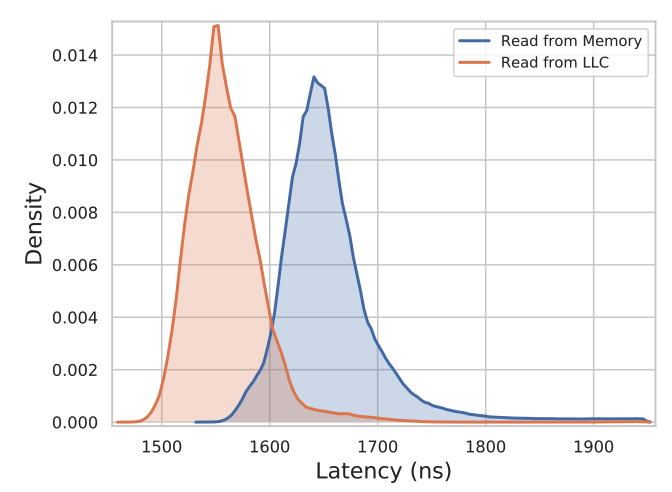
\includegraphics[width=\textwidth]{replication_graph.png}
\end{frame}

\begin{frame}
 \frametitle{Accomplishments}

 \begin{itemize}
  \item \textit{Probably} able to measure if a remote memory access is served from LLC or DRAM.
  \item Didn't get much farther as we struggled to get consistent results.
  \item Project became far more learning based than result based.
  \item Learned quite a lot about RDMA, Infiniband, DDIO, caches, CPU scaling, timing, etc.
 \end{itemize}

\end{frame}

\begin{frame}
 \frametitle{RDMA Overview}

 \begin{enumerate}
  \item Server and client both register memory to be used for RDMA.
 \end{enumerate}

 \begin{block}{Reads}
  \begin{enumerate}
   \setcounter{enumi}{1}
   \item Client specifies a remote address and fires off `READ' verb.
   \item Client NIC communicates with remote NIC to read remote memory address (no CPU involvement).
   \item Client NIC places remote memory contents into client's registered memory.
  \end{enumerate}
 \end{block}

 \begin{block}{Writes}
  \begin{enumerate}
   \setcounter{enumi}{1}
   \item Client alters local registered memory.
   \item Client specifies a remote address and fires off `WRITE' verb.
   \item Client NIC communicates with remote NIC to write local memory contents at remote address (no CPU involvement).
  \end{enumerate}
 \end{block}

\end{frame}

\begin{frame}
 \frametitle{Other Key Facts}

 \begin{block}{DDIO}
  \begin{itemize}
   \item Reads can be served from LLC or DRAM. If served from DRAM, the memory is \textbf{not} loaded into LLC.
   \item Writes will load memory into the LLC if not already present.
   \item DDIO is ``restricted to 10\% of the last-level cache''.
  \end{itemize}
 \end{block}

 \begin{block}{Infiniband}
  \begin{itemize}
   \item DRAM access and LLC access for an Infiniband NIC should take longer than a CPU's access due to PCIe communication?
   \item Infiniband RDMA reads (on \texttt{apt080} and \texttt{apt083}) take 1900ns on average with 50ns standard deviation.
  \end{itemize}
 \end{block}
\end{frame}

\begin{frame}
 \frametitle{Test Hardware}
 \begin{enumerate}
  \item Apt Cluster \texttt{r320}: 1 x Xeon E5-2450 processor (8 cores, 2.1Ghz), 16GB Memory (4 x 2GB RDIMMs, 1.6Ghz), 1 x Mellanox MX354A Dual port FDR CX3 adapter w/1 x QSA adapter
  \item Apt Cluster \texttt{c6220}: 2 x Xeon E5-2650v2 processors (8 cores each, 2.6Ghz), 64GB Memory (8 x 8GB DDR-3 RDIMMs, 1.86Ghz), 1 x Mellanox FDR CX3 Single port mezz card
  \item Notchpeak Cluster \texttt{notch010}: 2 x Intel(R) Xeon(R) Gold 6130 CPU @ 2.10GHz, 186GB Memory, EDR Infiniband
 \end{enumerate}

\end{frame}

\begin{frame}[fragile]
 \frametitle{Timing Code}
 Let $x$ be a remote address.
 \begin{enumerate}
  \item Read $x$ (cache miss)
  \item Write to $x$ (pull into cache)
  \item Read $x$ (cache hit)
 \end{enumerate}

 \begin{lstlisting}[frame=single,language=C,basicstyle=\tiny]
start_cycle_count = start_tsc(); // lfence -> rdtsc -> lfence

rc = ibv_post_send(res->qp, &sr, &bad_wr);
if (rc)
    fprintf(stderr, "failed to post SR\n");
do {
    poll_result = ibv_poll_cq(res->cq, 1, &wc);
} while (poll_result == 0);

end_cycle_count = stop_tsc(); // rdtscp -> lfence
\end{lstlisting}
 \footnotesize
 \texttt{start\_tsc}/\texttt{stop\_tsc} code taken from Google's Highway Hash Git repo.
\end{frame}

\begin{frame}
 \frametitle{Read-Write-Read Methods}

 \vskip0pt plus 1filll
 \begin{enumerate}
  \item Read-write-read single address with a \texttt{clflush} between each iteration
  \item Sequential reads with strides to (hopefully) overcome any prefetchers

         {\tiny (64 byte msgs, columns count = 4, row count = 524288, {\raise.17ex\hbox{$\scriptstyle\mathtt{\sim}$}}134 MB total)}
  \item Random access
 \end{enumerate}

 \vskip0pt plus 1filll
 \begin{block}{\footnotesize{}Data Note}
  \footnotesize
  Graphs, unless noted, filter out data points where the diff was negative or the diff was $>=$ 99 percentile.
  Graphs generated with \texttt{ggplot2} in \texttt{R}.
 \end{block}
 \vspace{20pt}
\end{frame}

\begin{frame}[t,fragile]
 \frametitle{\texttt{clflush} Method}
 Client read$\rightarrow$write$\rightarrow$reads then syncs with server to call \texttt{clflush}.

 \begin{block}{Client Code}

  \begin{lstlisting}[frame=single, language=C, basicstyle=\tiny]
for (i = 0; i < iters; ++i) {
    if (read_write_read(&res, start_addr, cycles_to_usec)) { ... }

    if (sock_sync_data(res.sock, 1, "A", &temp_char)) { ... }

    if (sock_sync_data(res.sock, 1, "B", &temp_char)) { ... }
}
 \end{lstlisting}
 \end{block}

 \begin{block}{Server Code}
  \begin{lstlisting}[frame=single, language=C, basicstyle=\tiny]
for (i = 0; i < iters; ++i) {
    if (sock_sync_data(res.sock, 1, "A", &temp_char)) { ... }

    _mm_clflush(res.buf);
    _mm_mfence();

    if (sock_sync_data(res.sock, 1, "B", &temp_char)) { ... }
}
 \end{lstlisting}
 \end{block}

\end{frame}

\begin{frame}[fragile]
 \frametitle{\texttt{clflush} Method}
 \begin{columns}
  \begin{column}{0.5\textwidth}
   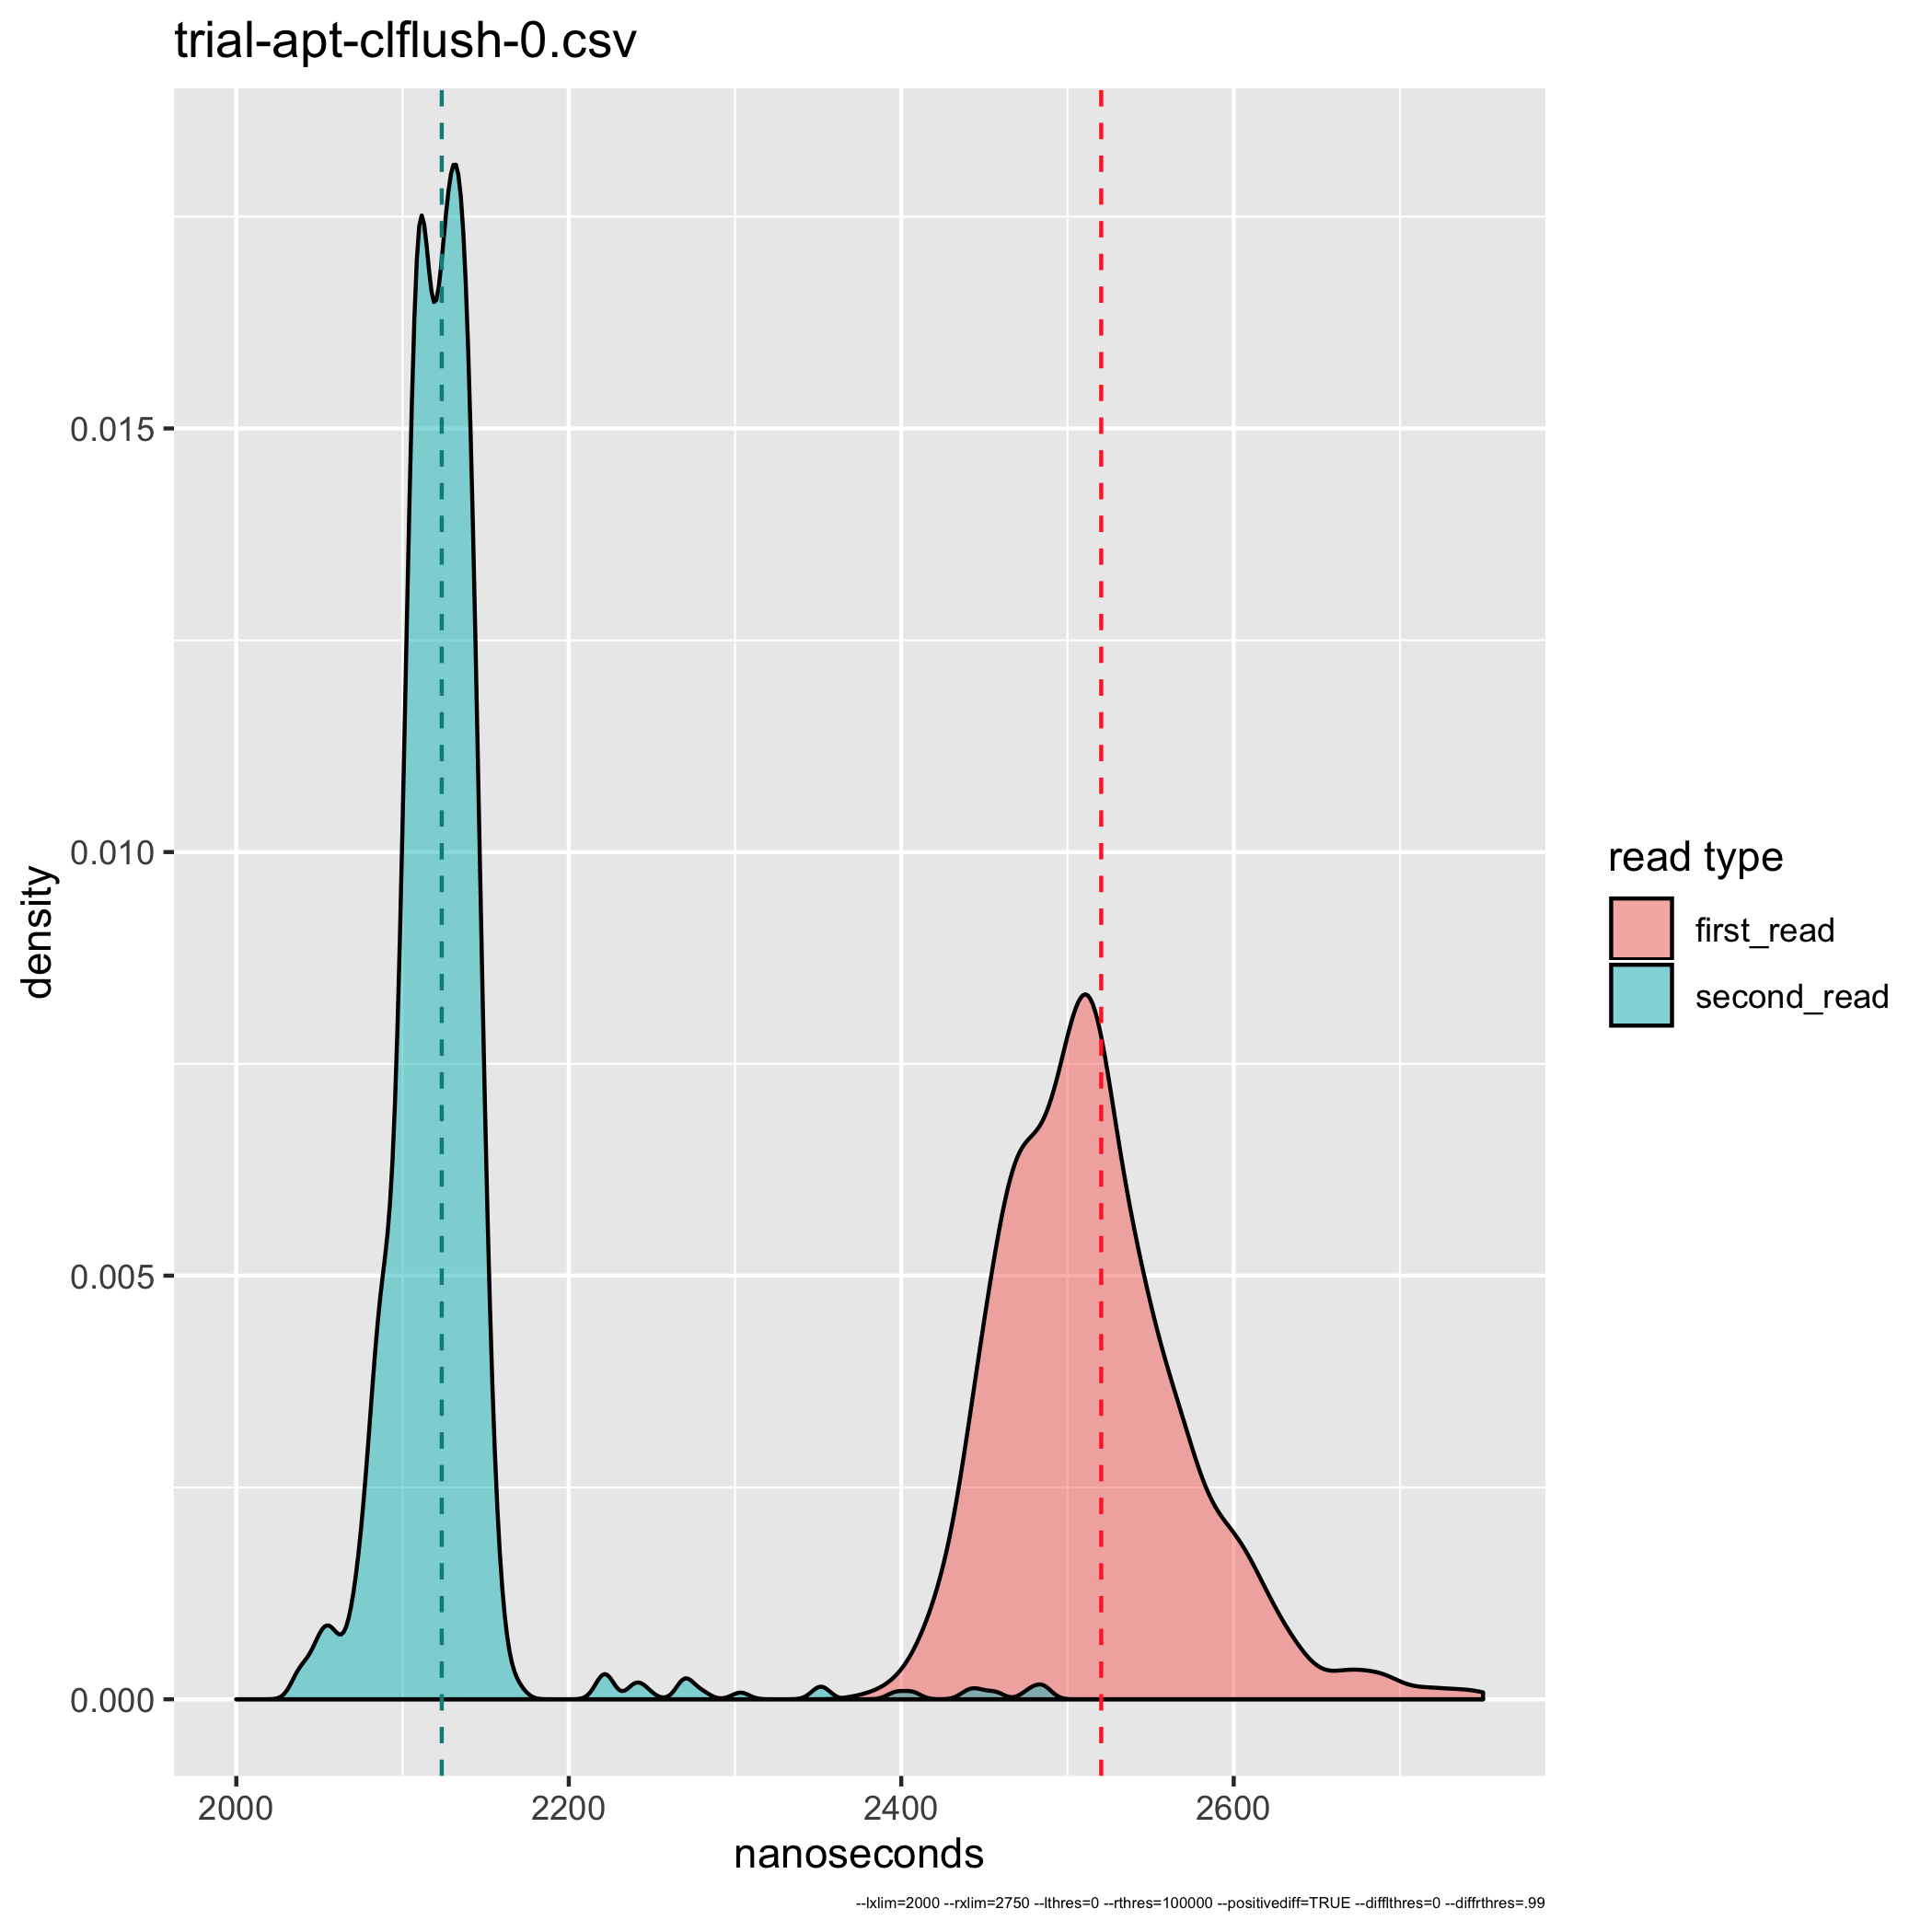
\includegraphics[width=\linewidth]{trial-apt-clflush-0-histogram.png}

  \end{column}
  \begin{column}{0.5\textwidth}
   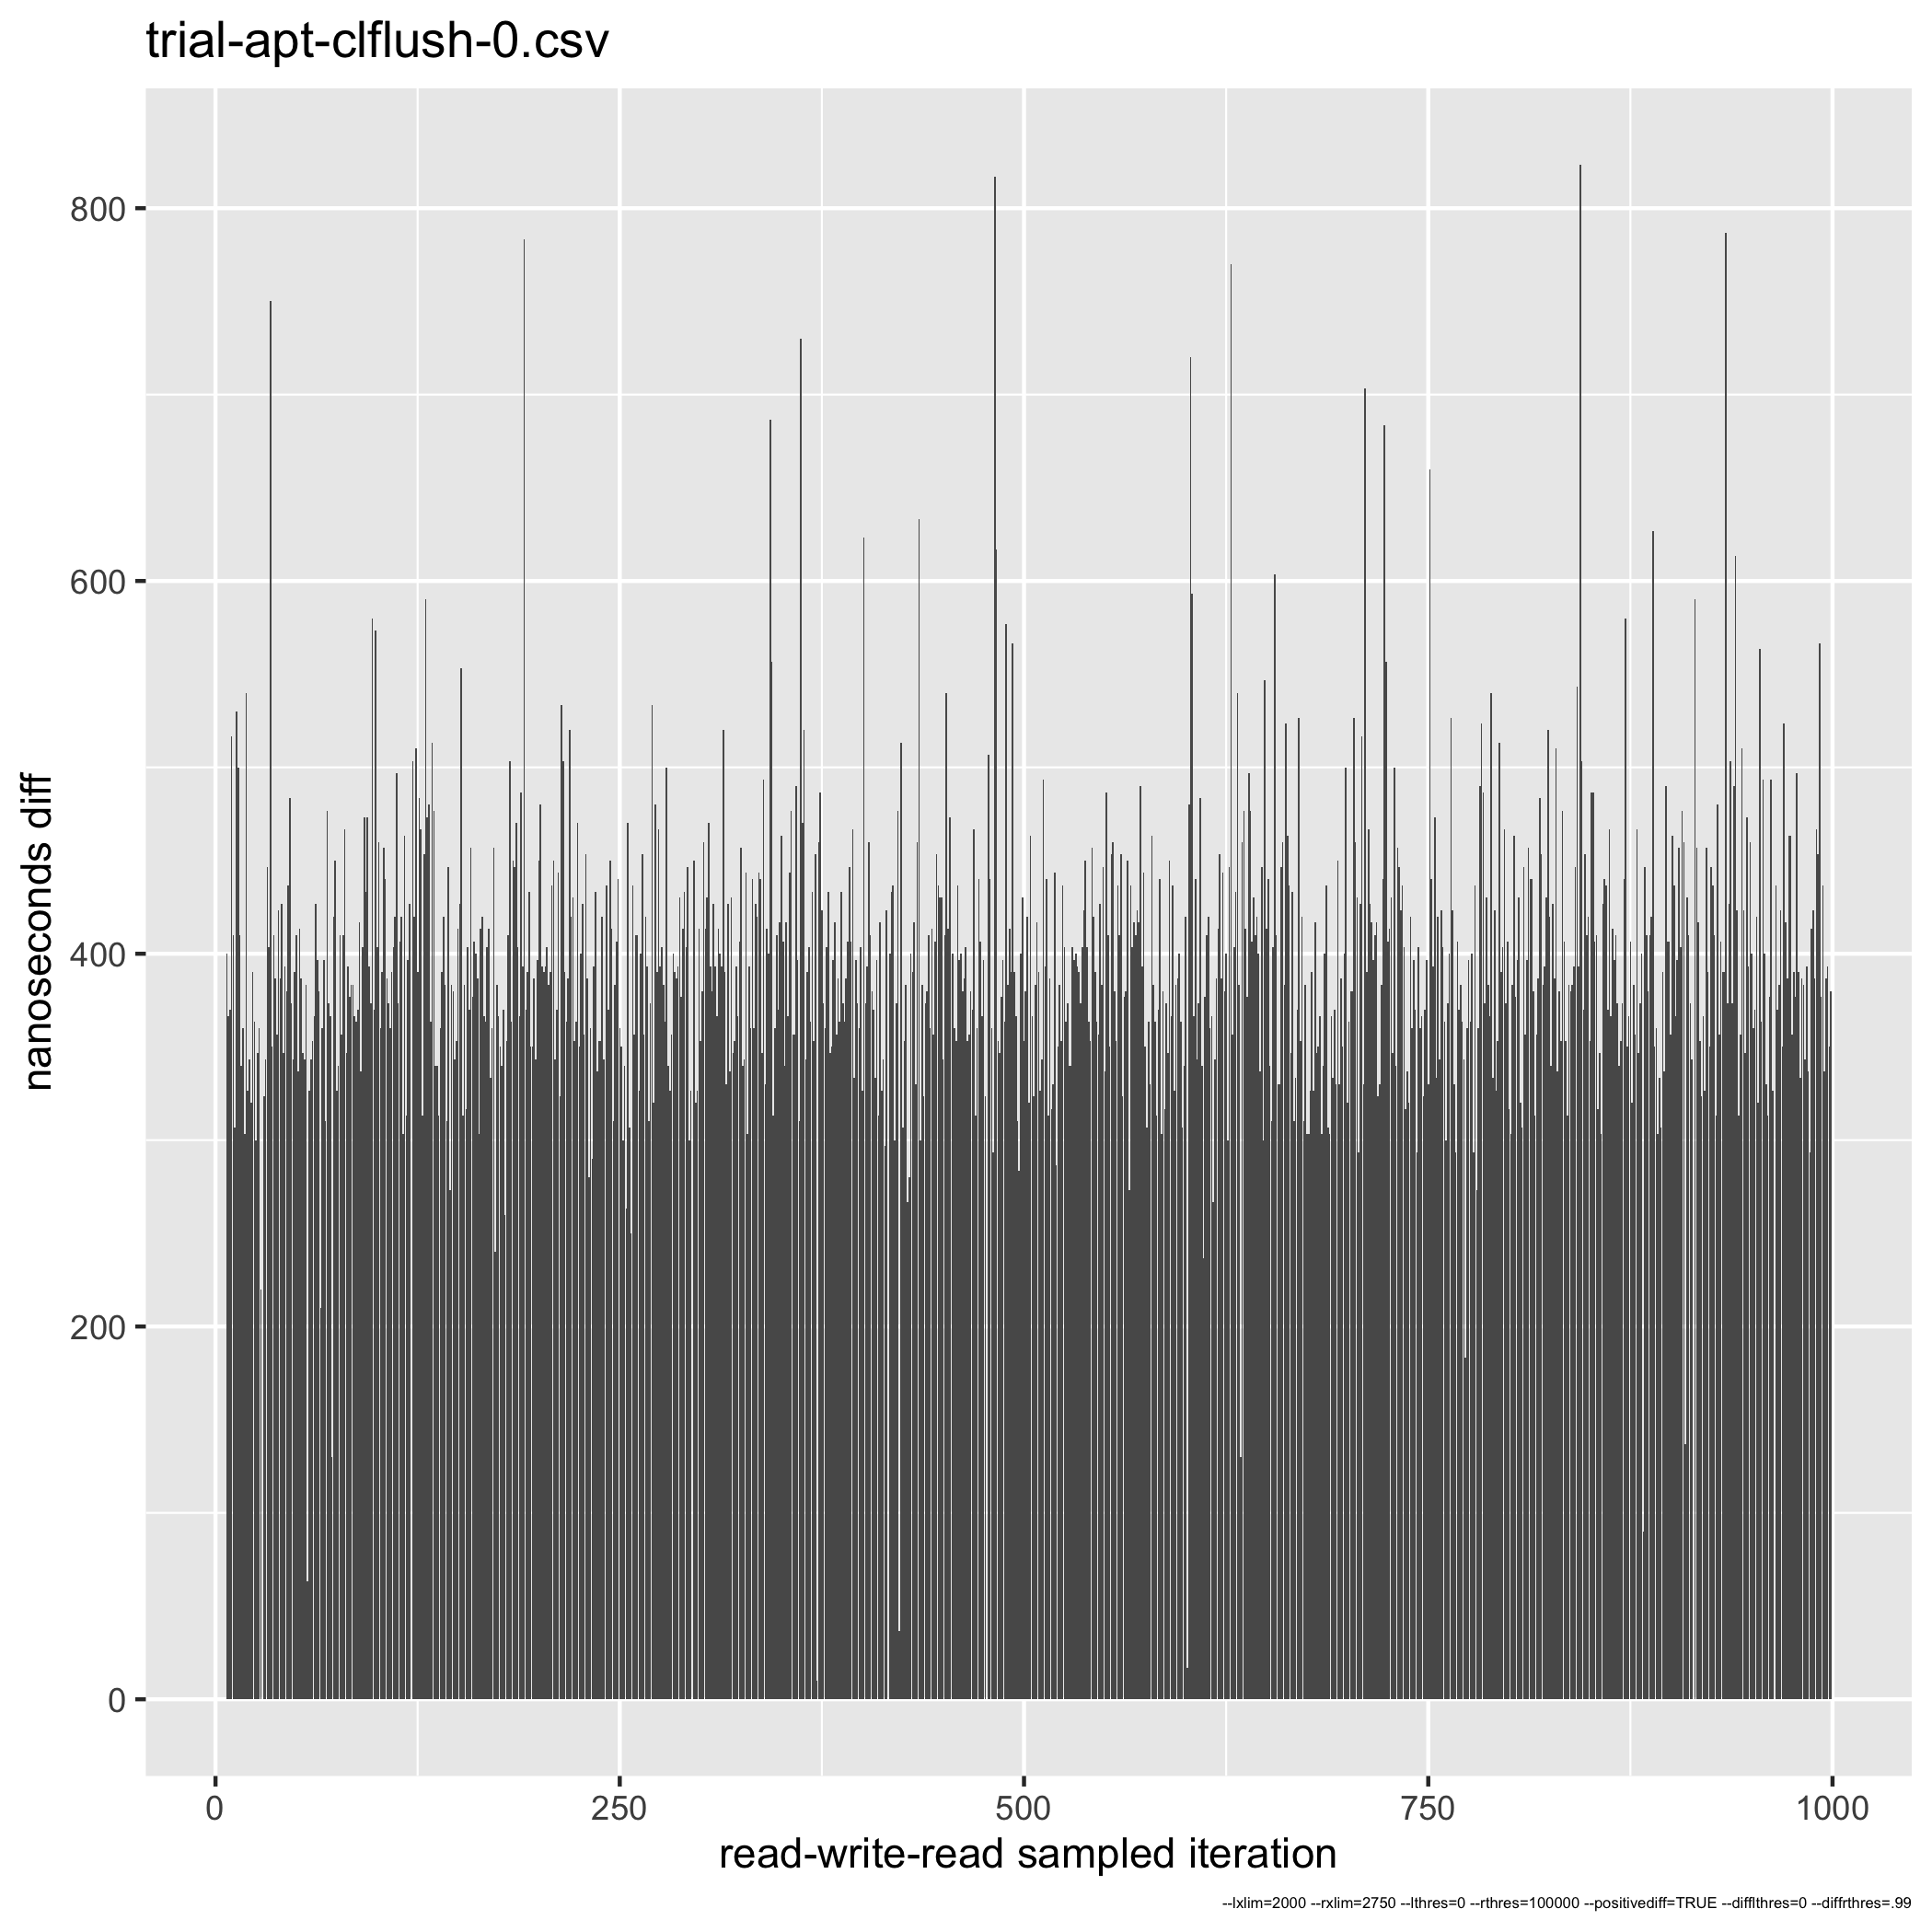
\includegraphics[width=\linewidth]{trial-apt-clflush-0-barchart.png}

  \end{column}

 \end{columns}
\end{frame}

\begin{frame}
 \frametitle{\texttt{clflush} Method}
 Calvin tried read$\rightarrow$read only... :(

 \vspace{10pt}
 \centering
 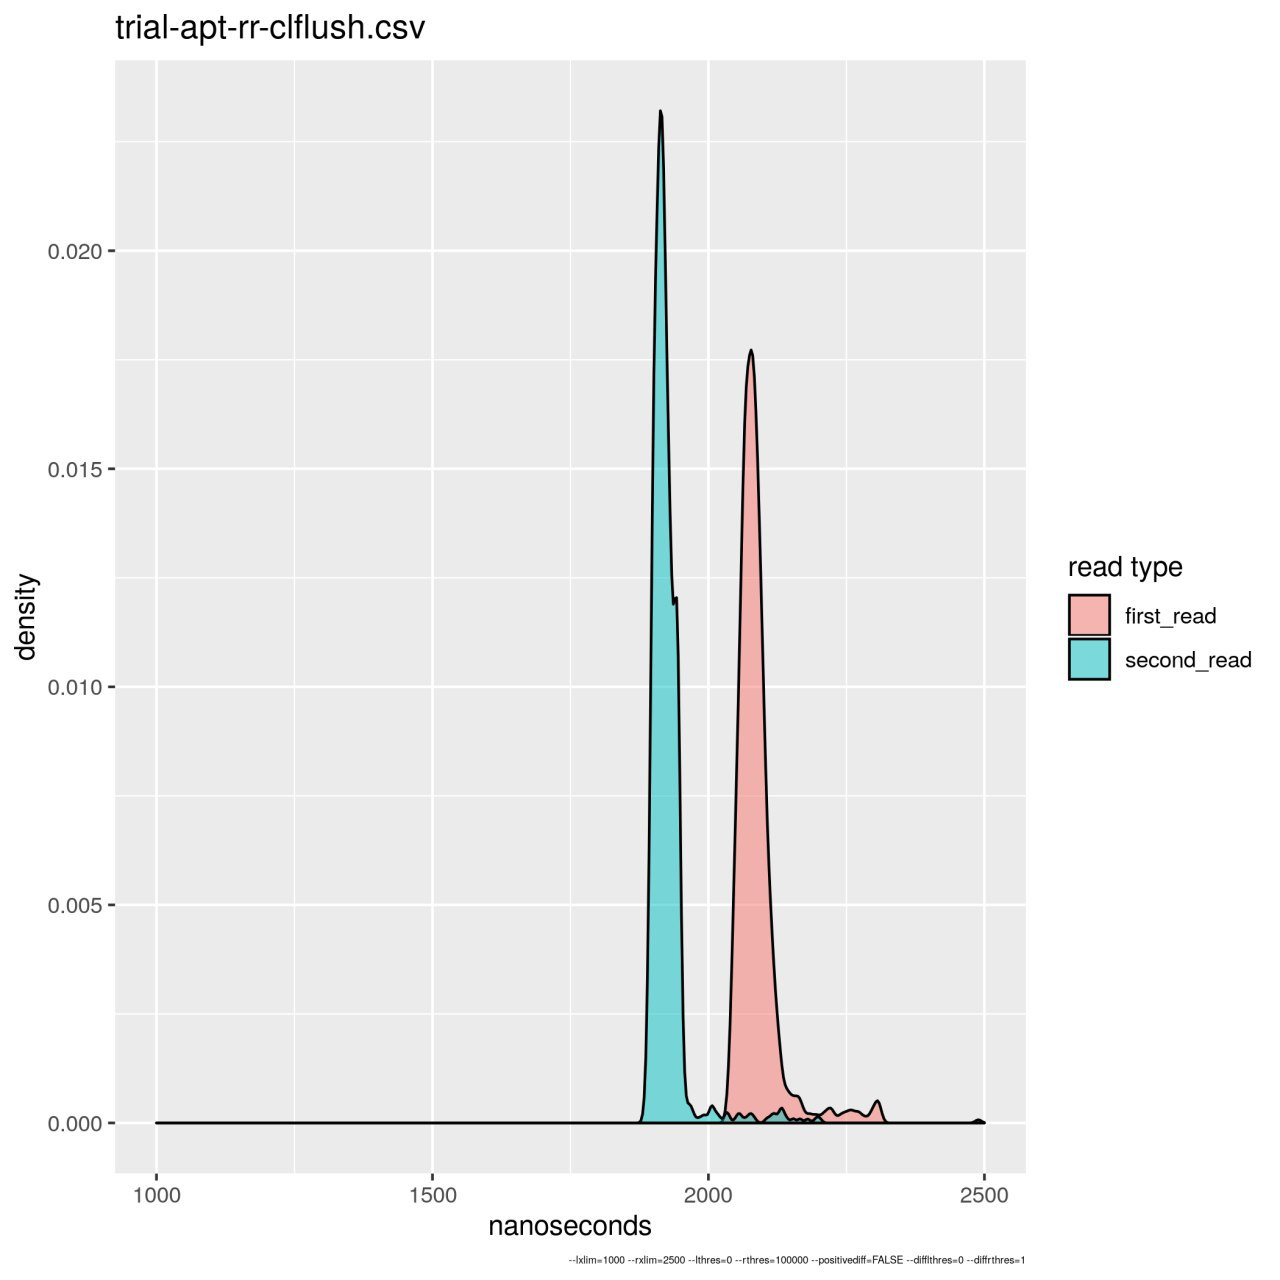
\includegraphics[height=\textheight - 20mm]{trial-apt-clflush-rr.jpg}

\end{frame}

\begin{frame}[t]
 \frametitle{\texttt{clflush} Method}
 And these happened a few times with read$\rightarrow$write$\rightarrow$read?

 \vspace{20pt}
 \begin{columns}
  \begin{column}{0.5\textwidth}
   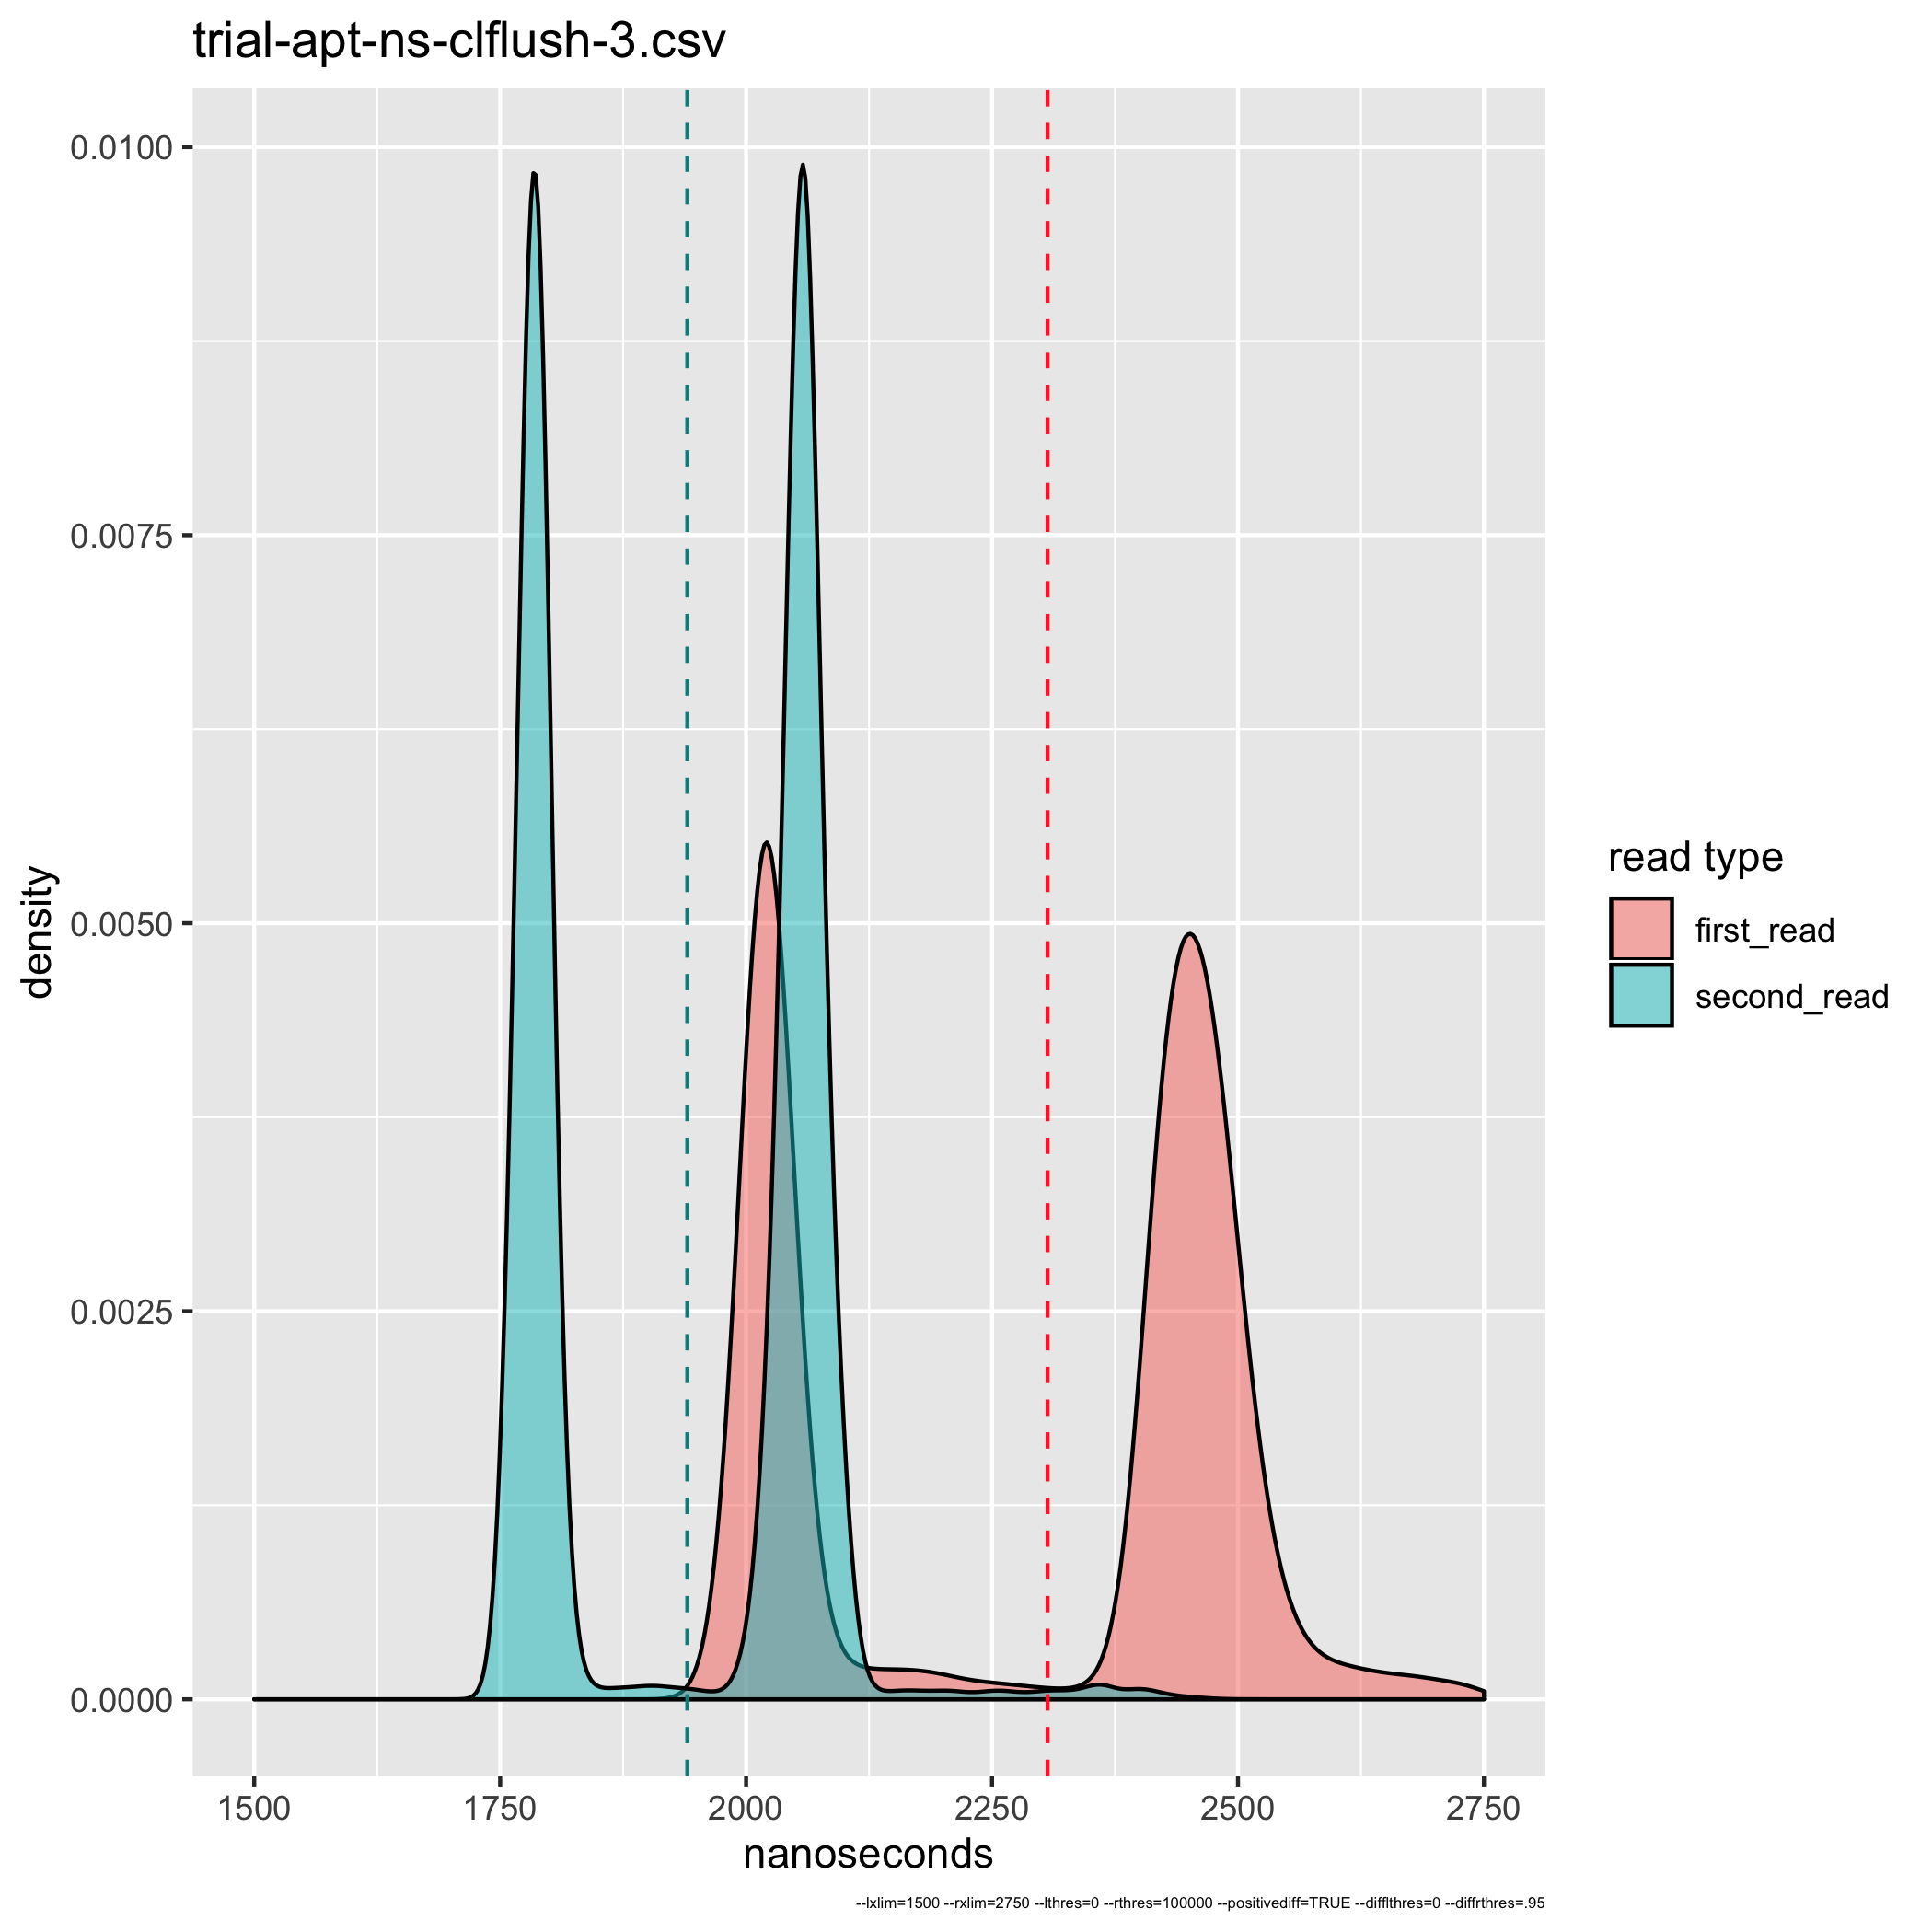
\includegraphics[width=\linewidth]{trial-apt-ns-clflush-3-histogram.png}

  \end{column}
  \begin{column}{0.5\textwidth}
   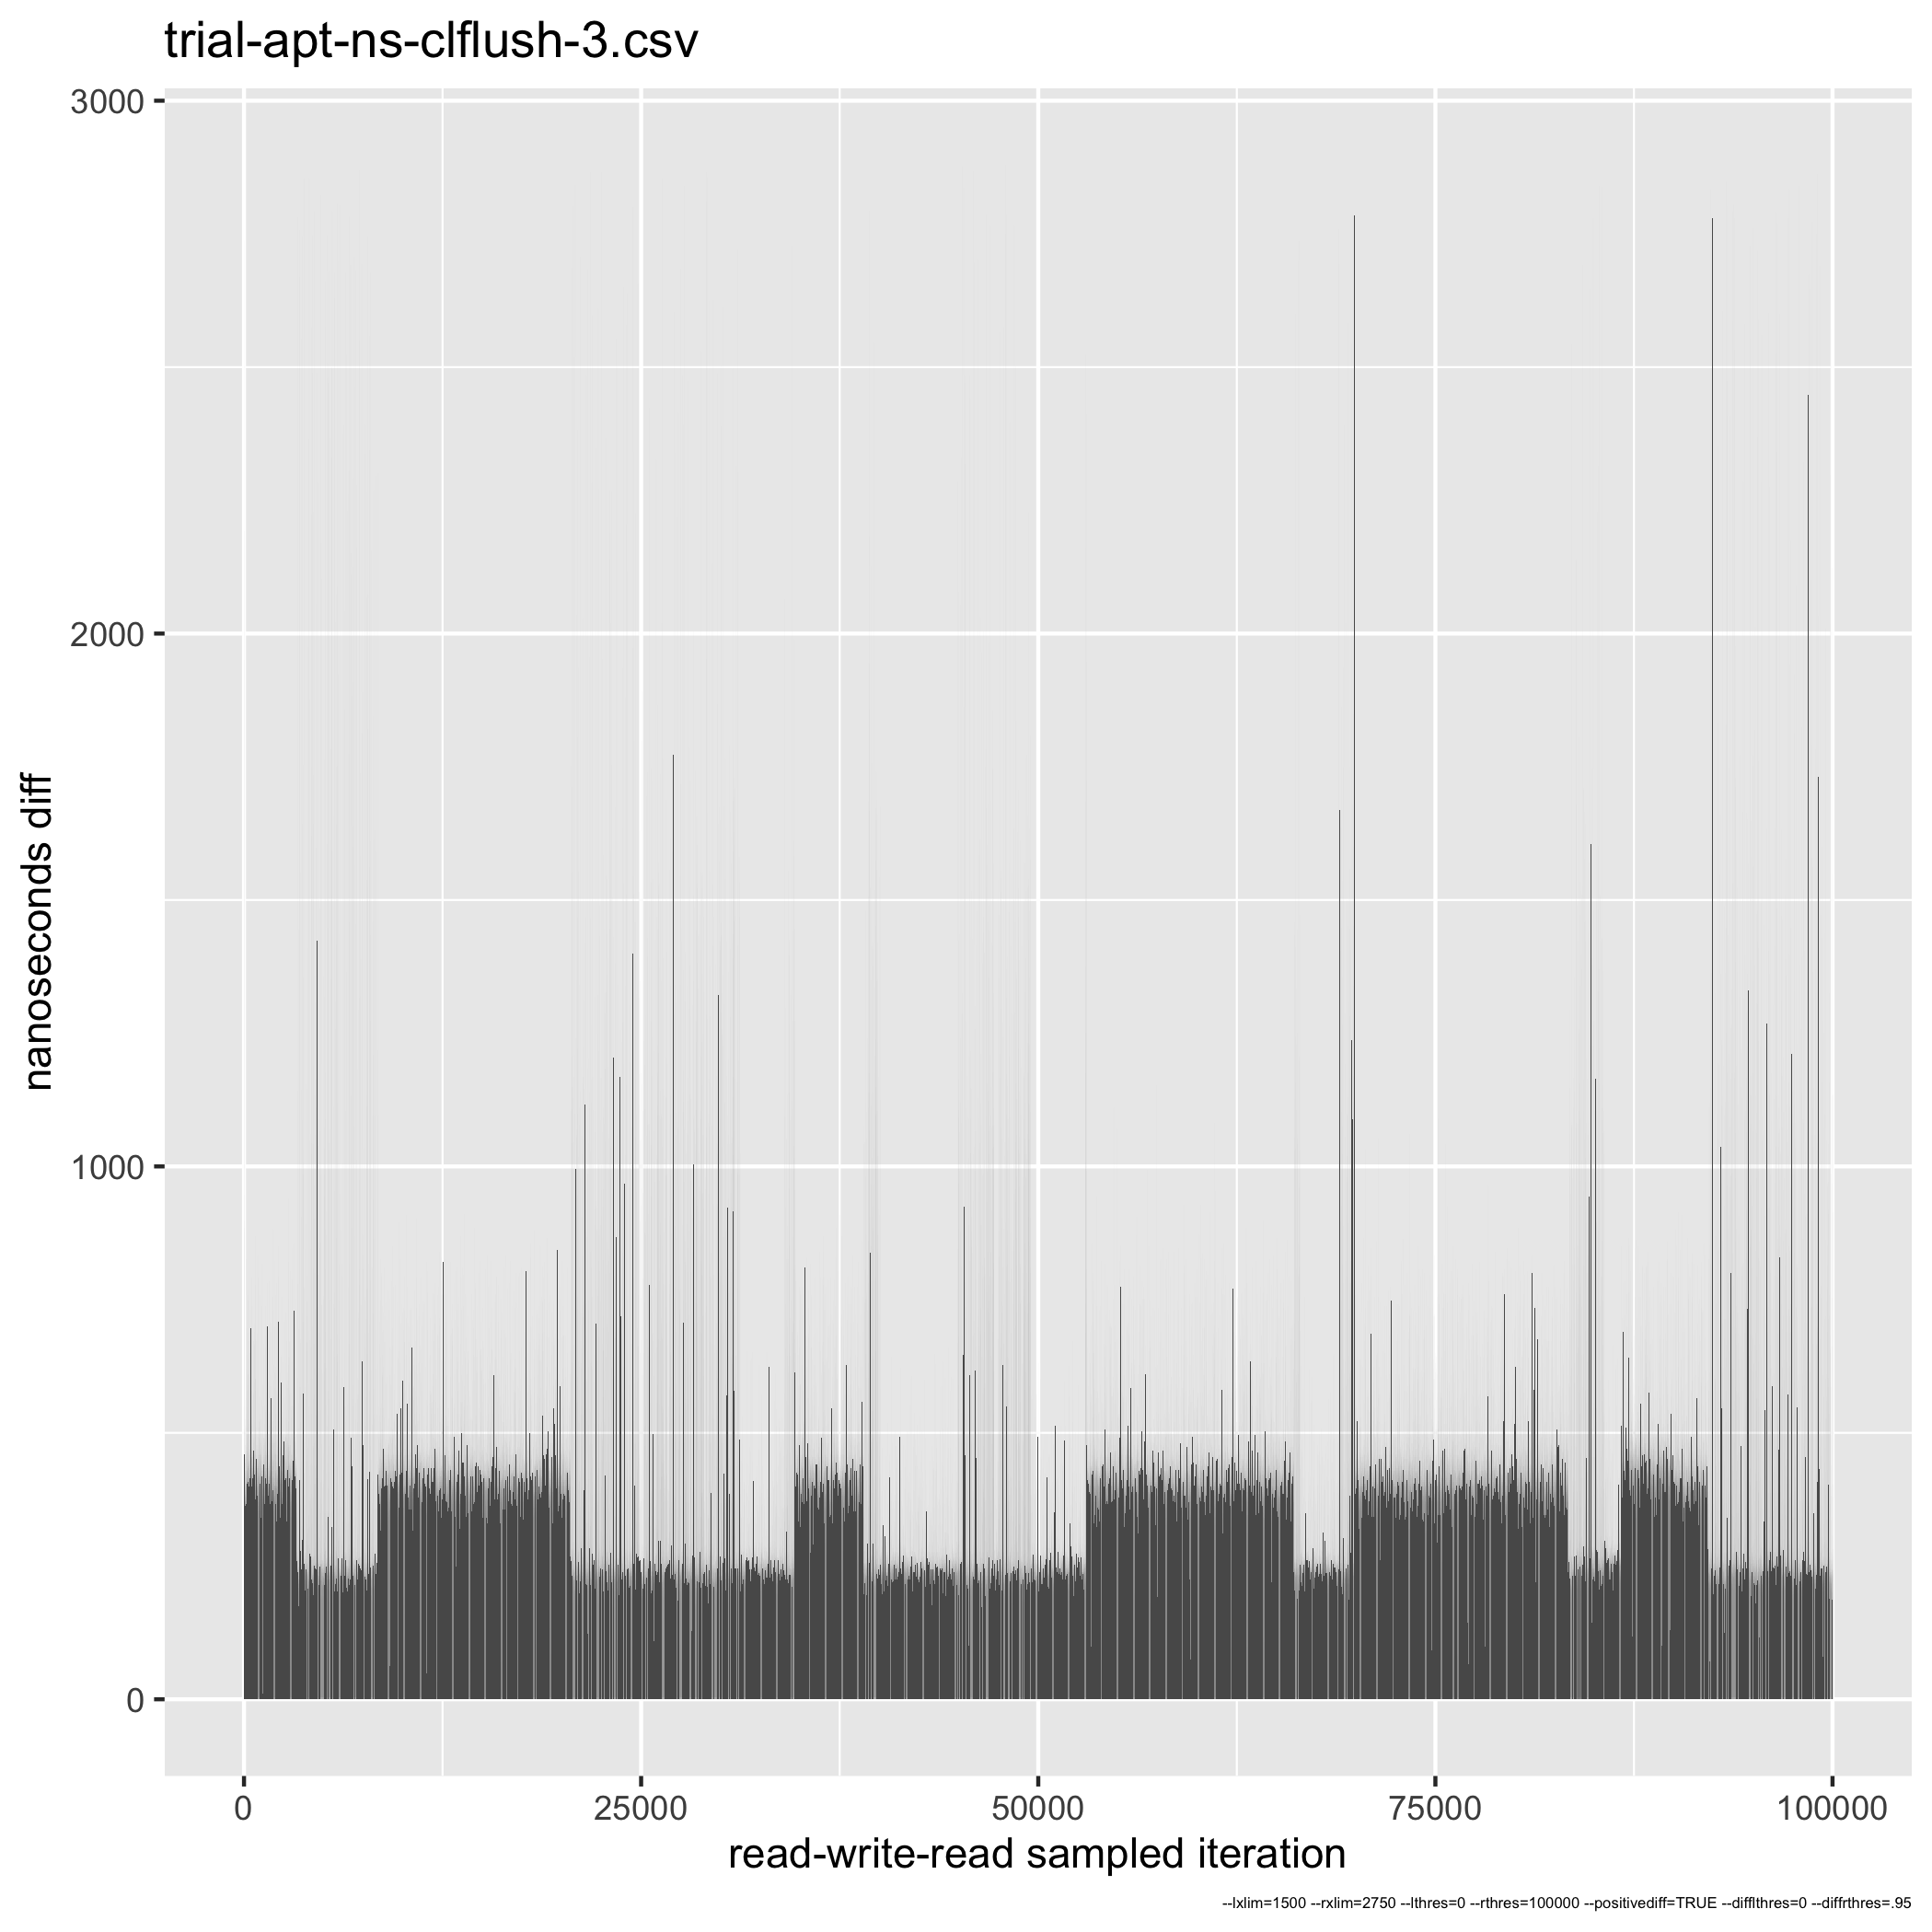
\includegraphics[width=\linewidth]{trial-apt-ns-clflush-3-barchart.png}

  \end{column}

 \end{columns}

\end{frame}


\begin{frame}
 \frametitle{Random Access Method}
 Tended to produce the cleanest data.
 \begin{columns}
  \begin{column}{0.5\textwidth}
   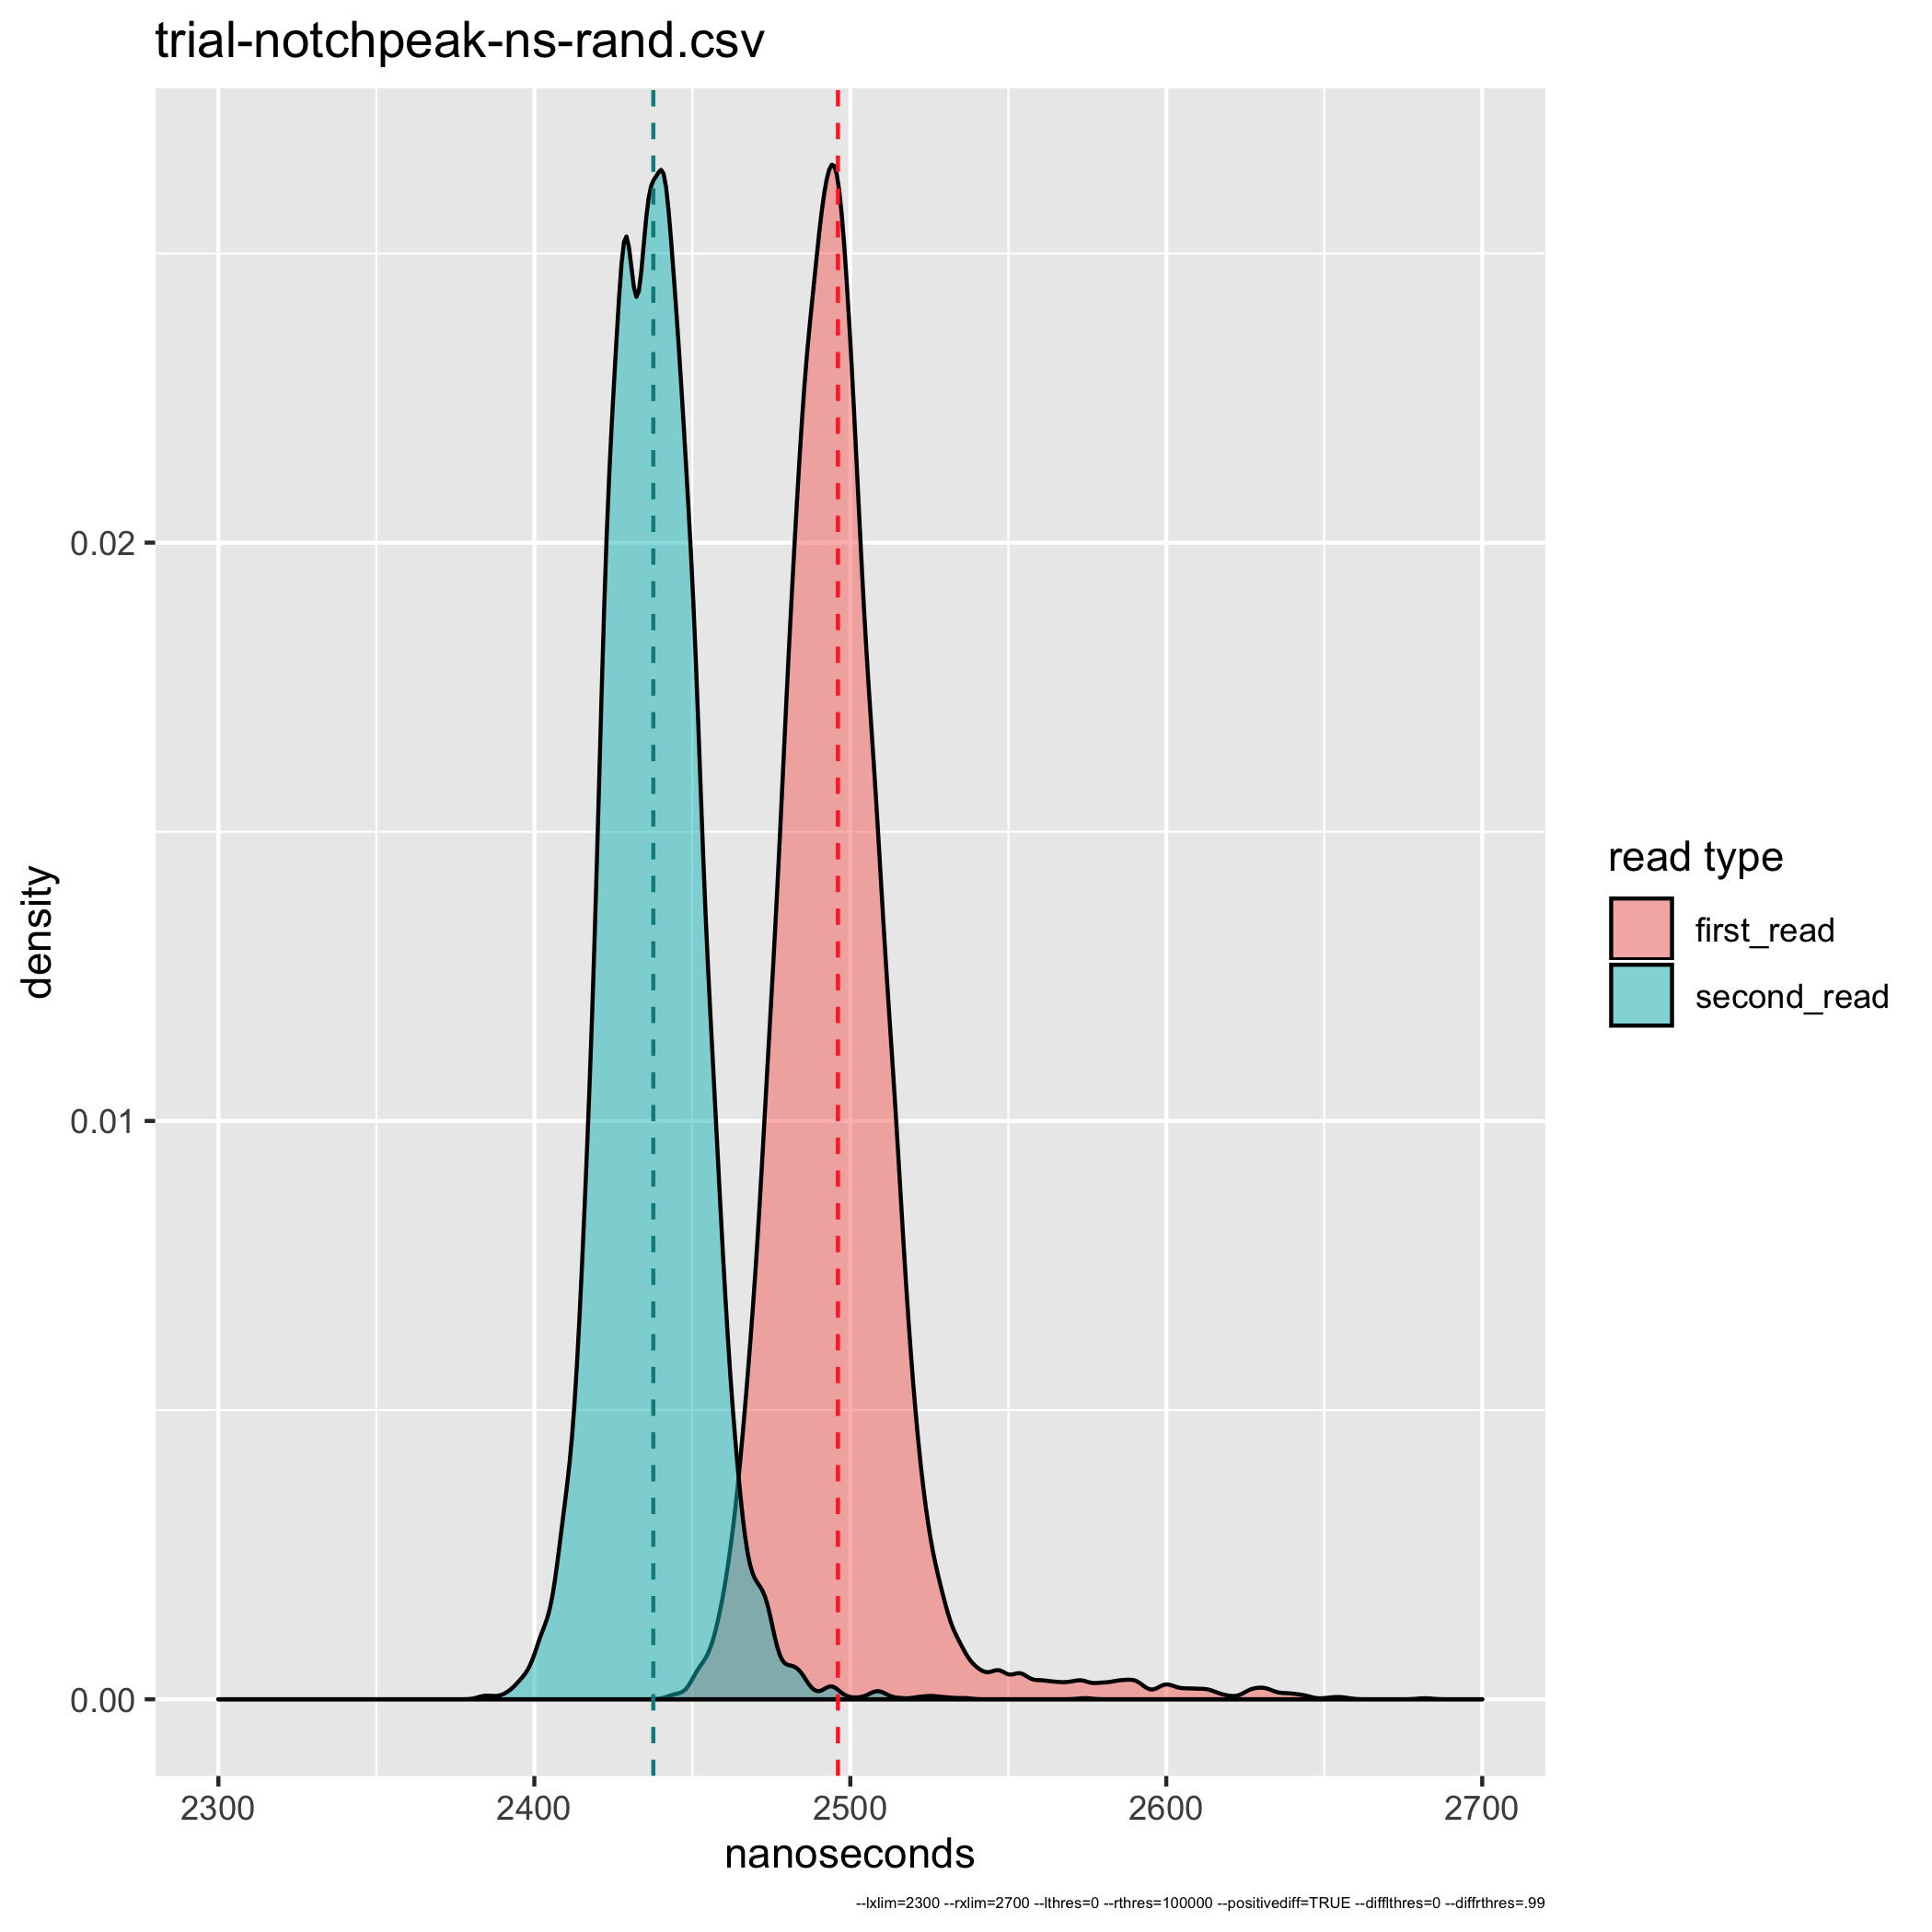
\includegraphics[width=\linewidth]{trial-notchpeak-ns-rand-histogram.png}

  \end{column}
  \begin{column}{0.5\textwidth}
   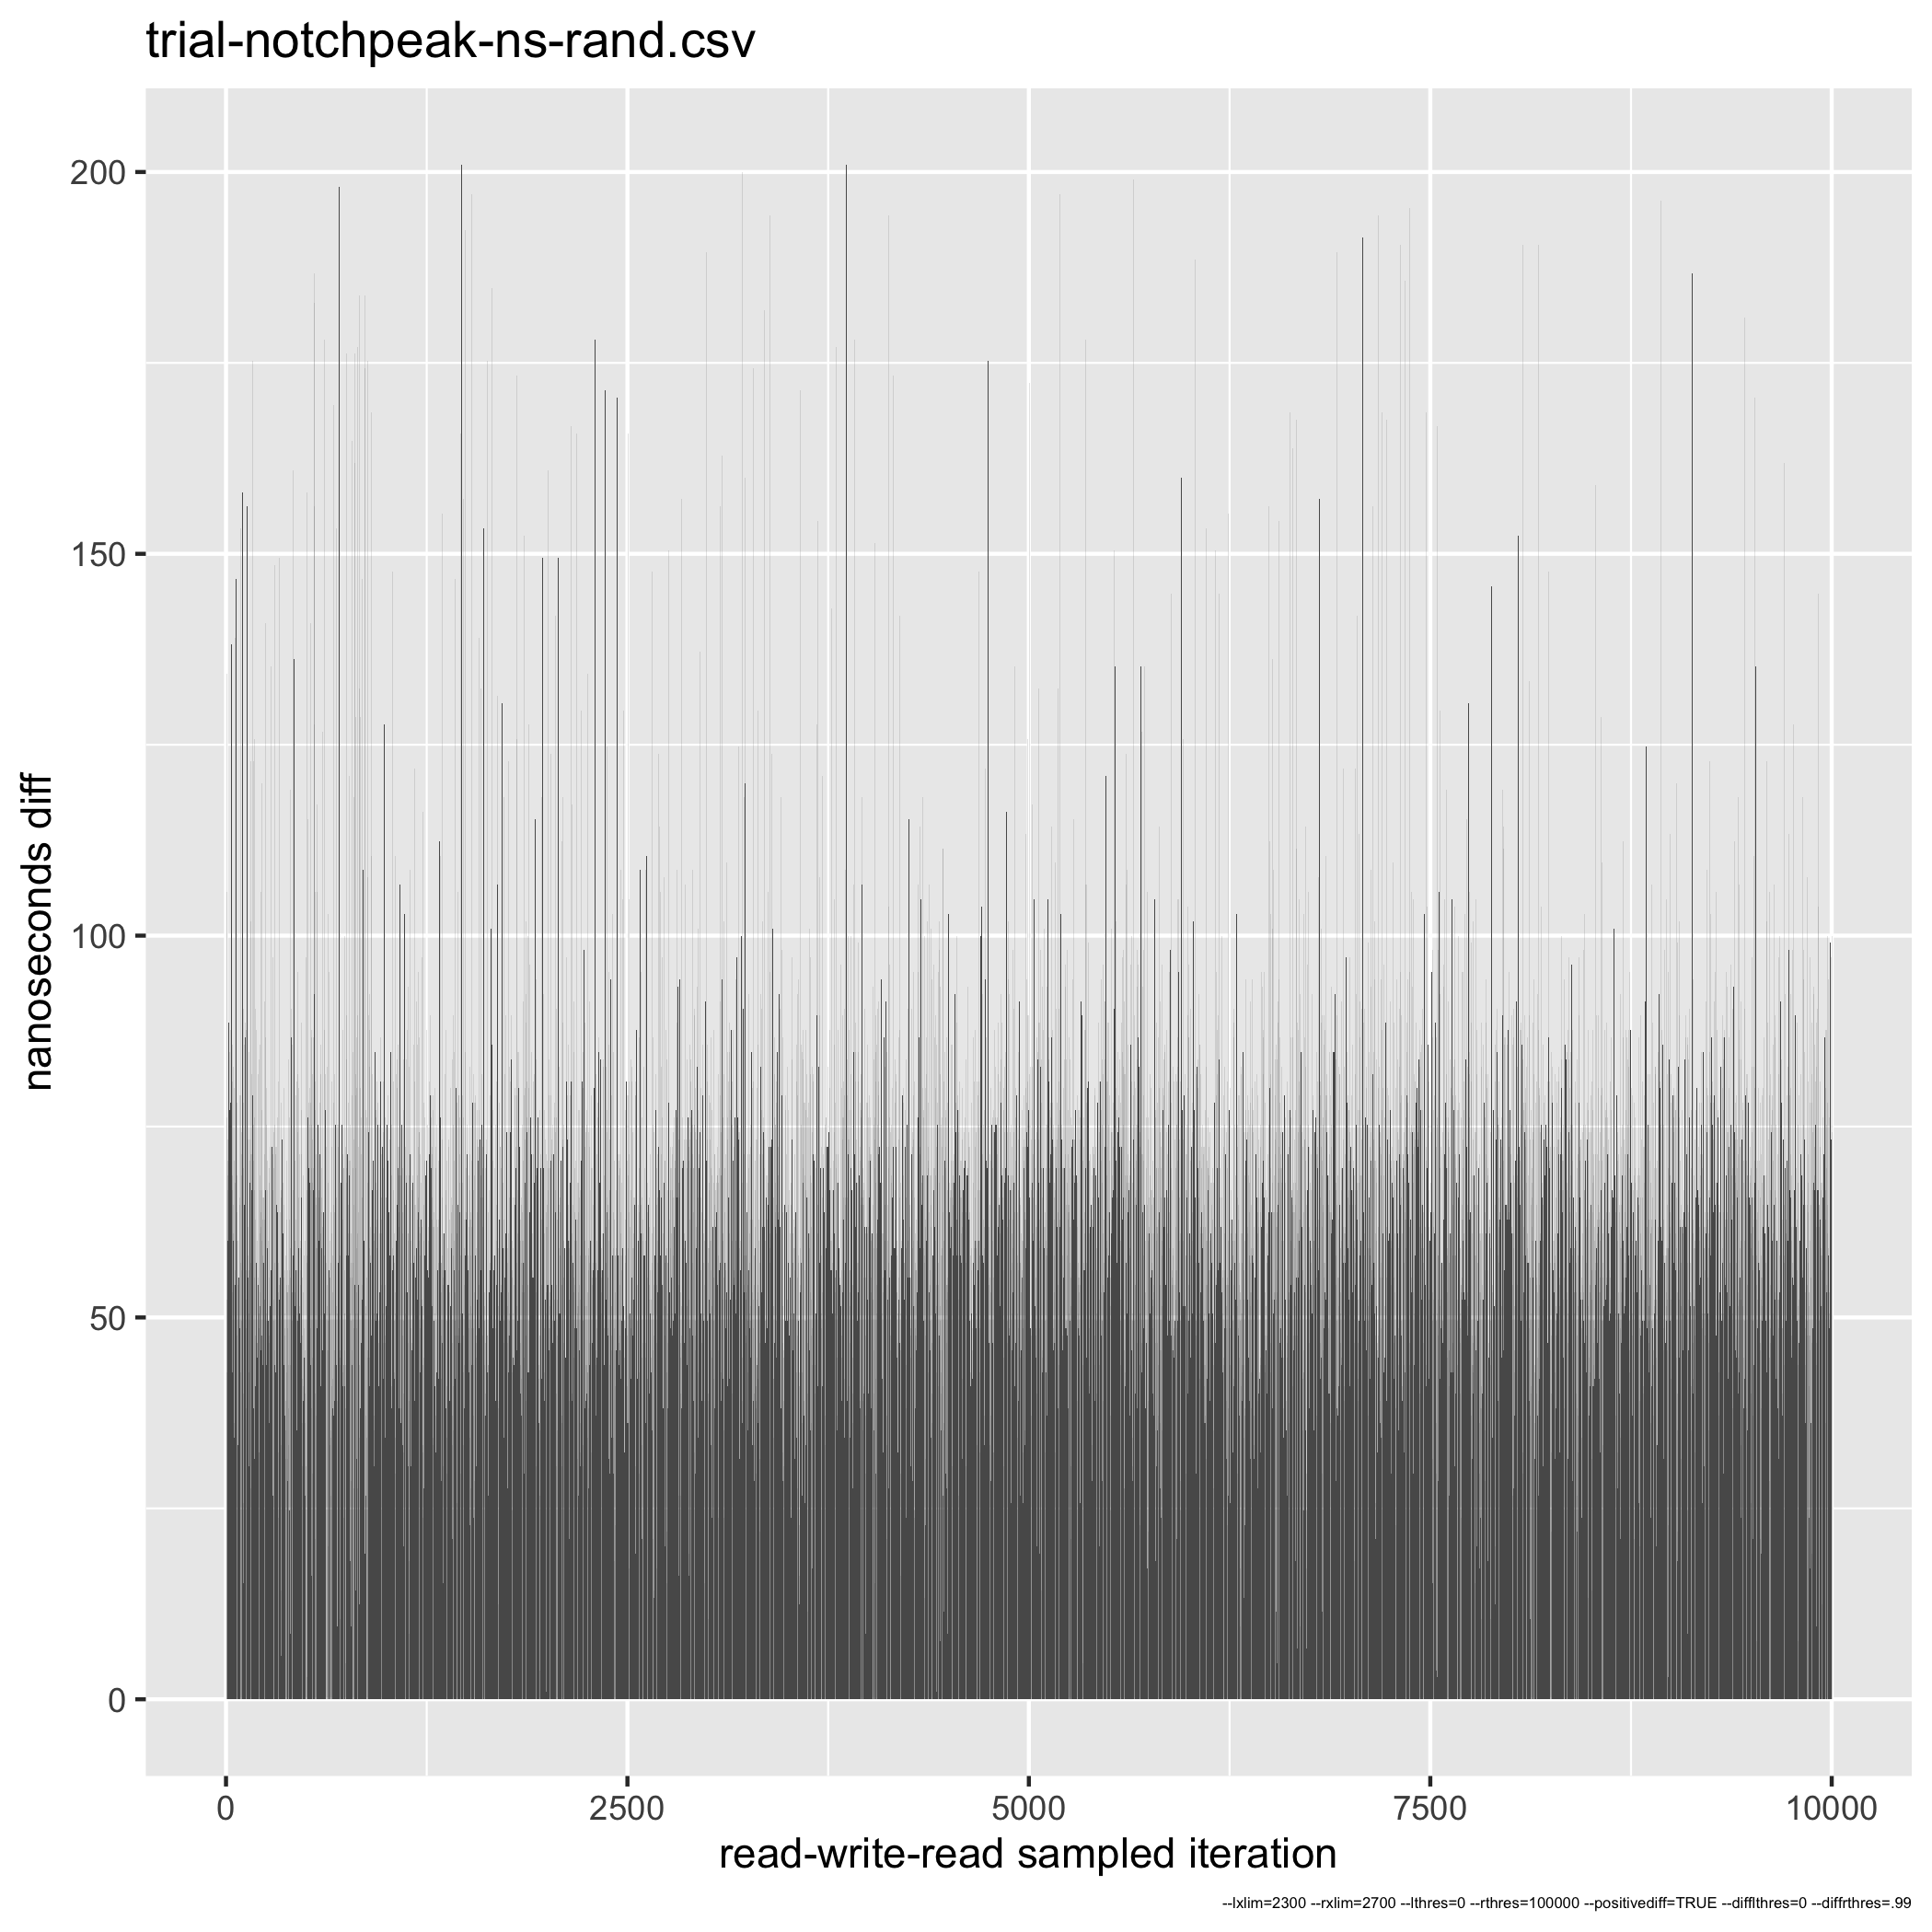
\includegraphics[width=\linewidth]{trial-notchpeak-ns-rand-barchart.png}

  \end{column}

 \end{columns}

\end{frame}

\begin{frame}
 \frametitle{Random Access Method}
 Sometimes the results came out flipped?
 \begin{columns}
  \begin{column}{0.5\textwidth}
   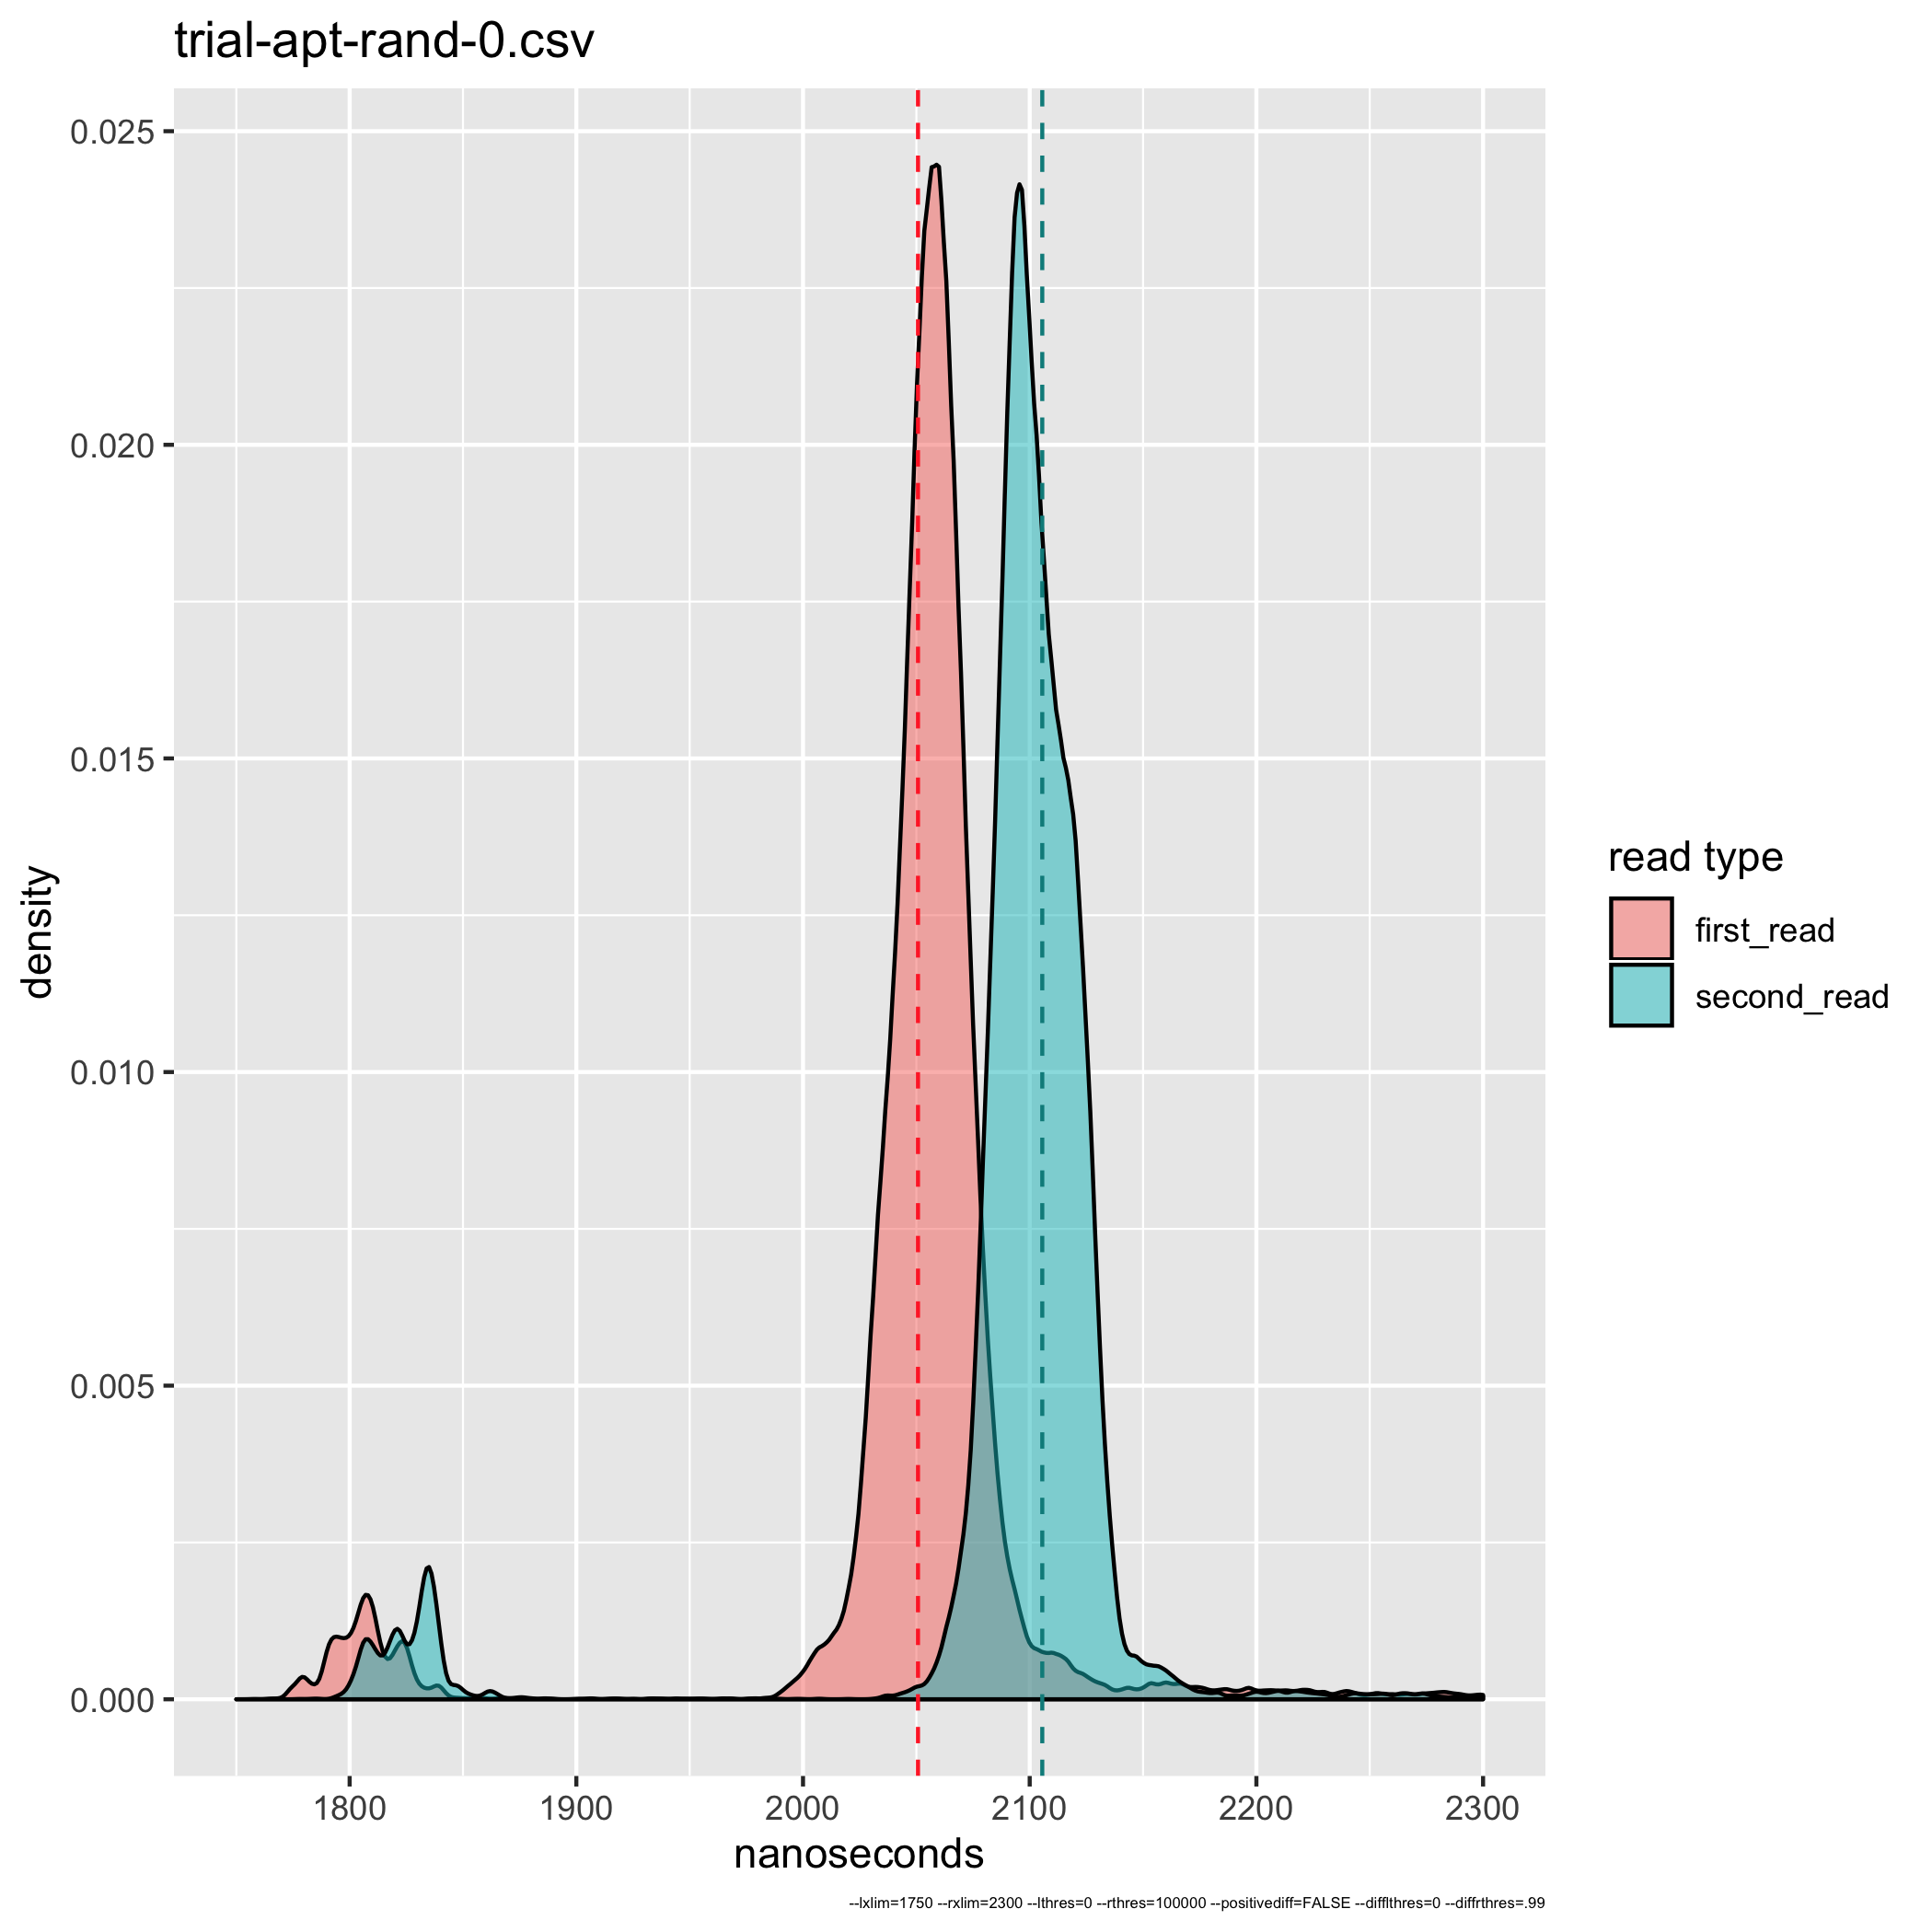
\includegraphics[width=\linewidth]{trial-apt-rand-0-histogram.png}

  \end{column}
  \begin{column}{0.5\textwidth}
   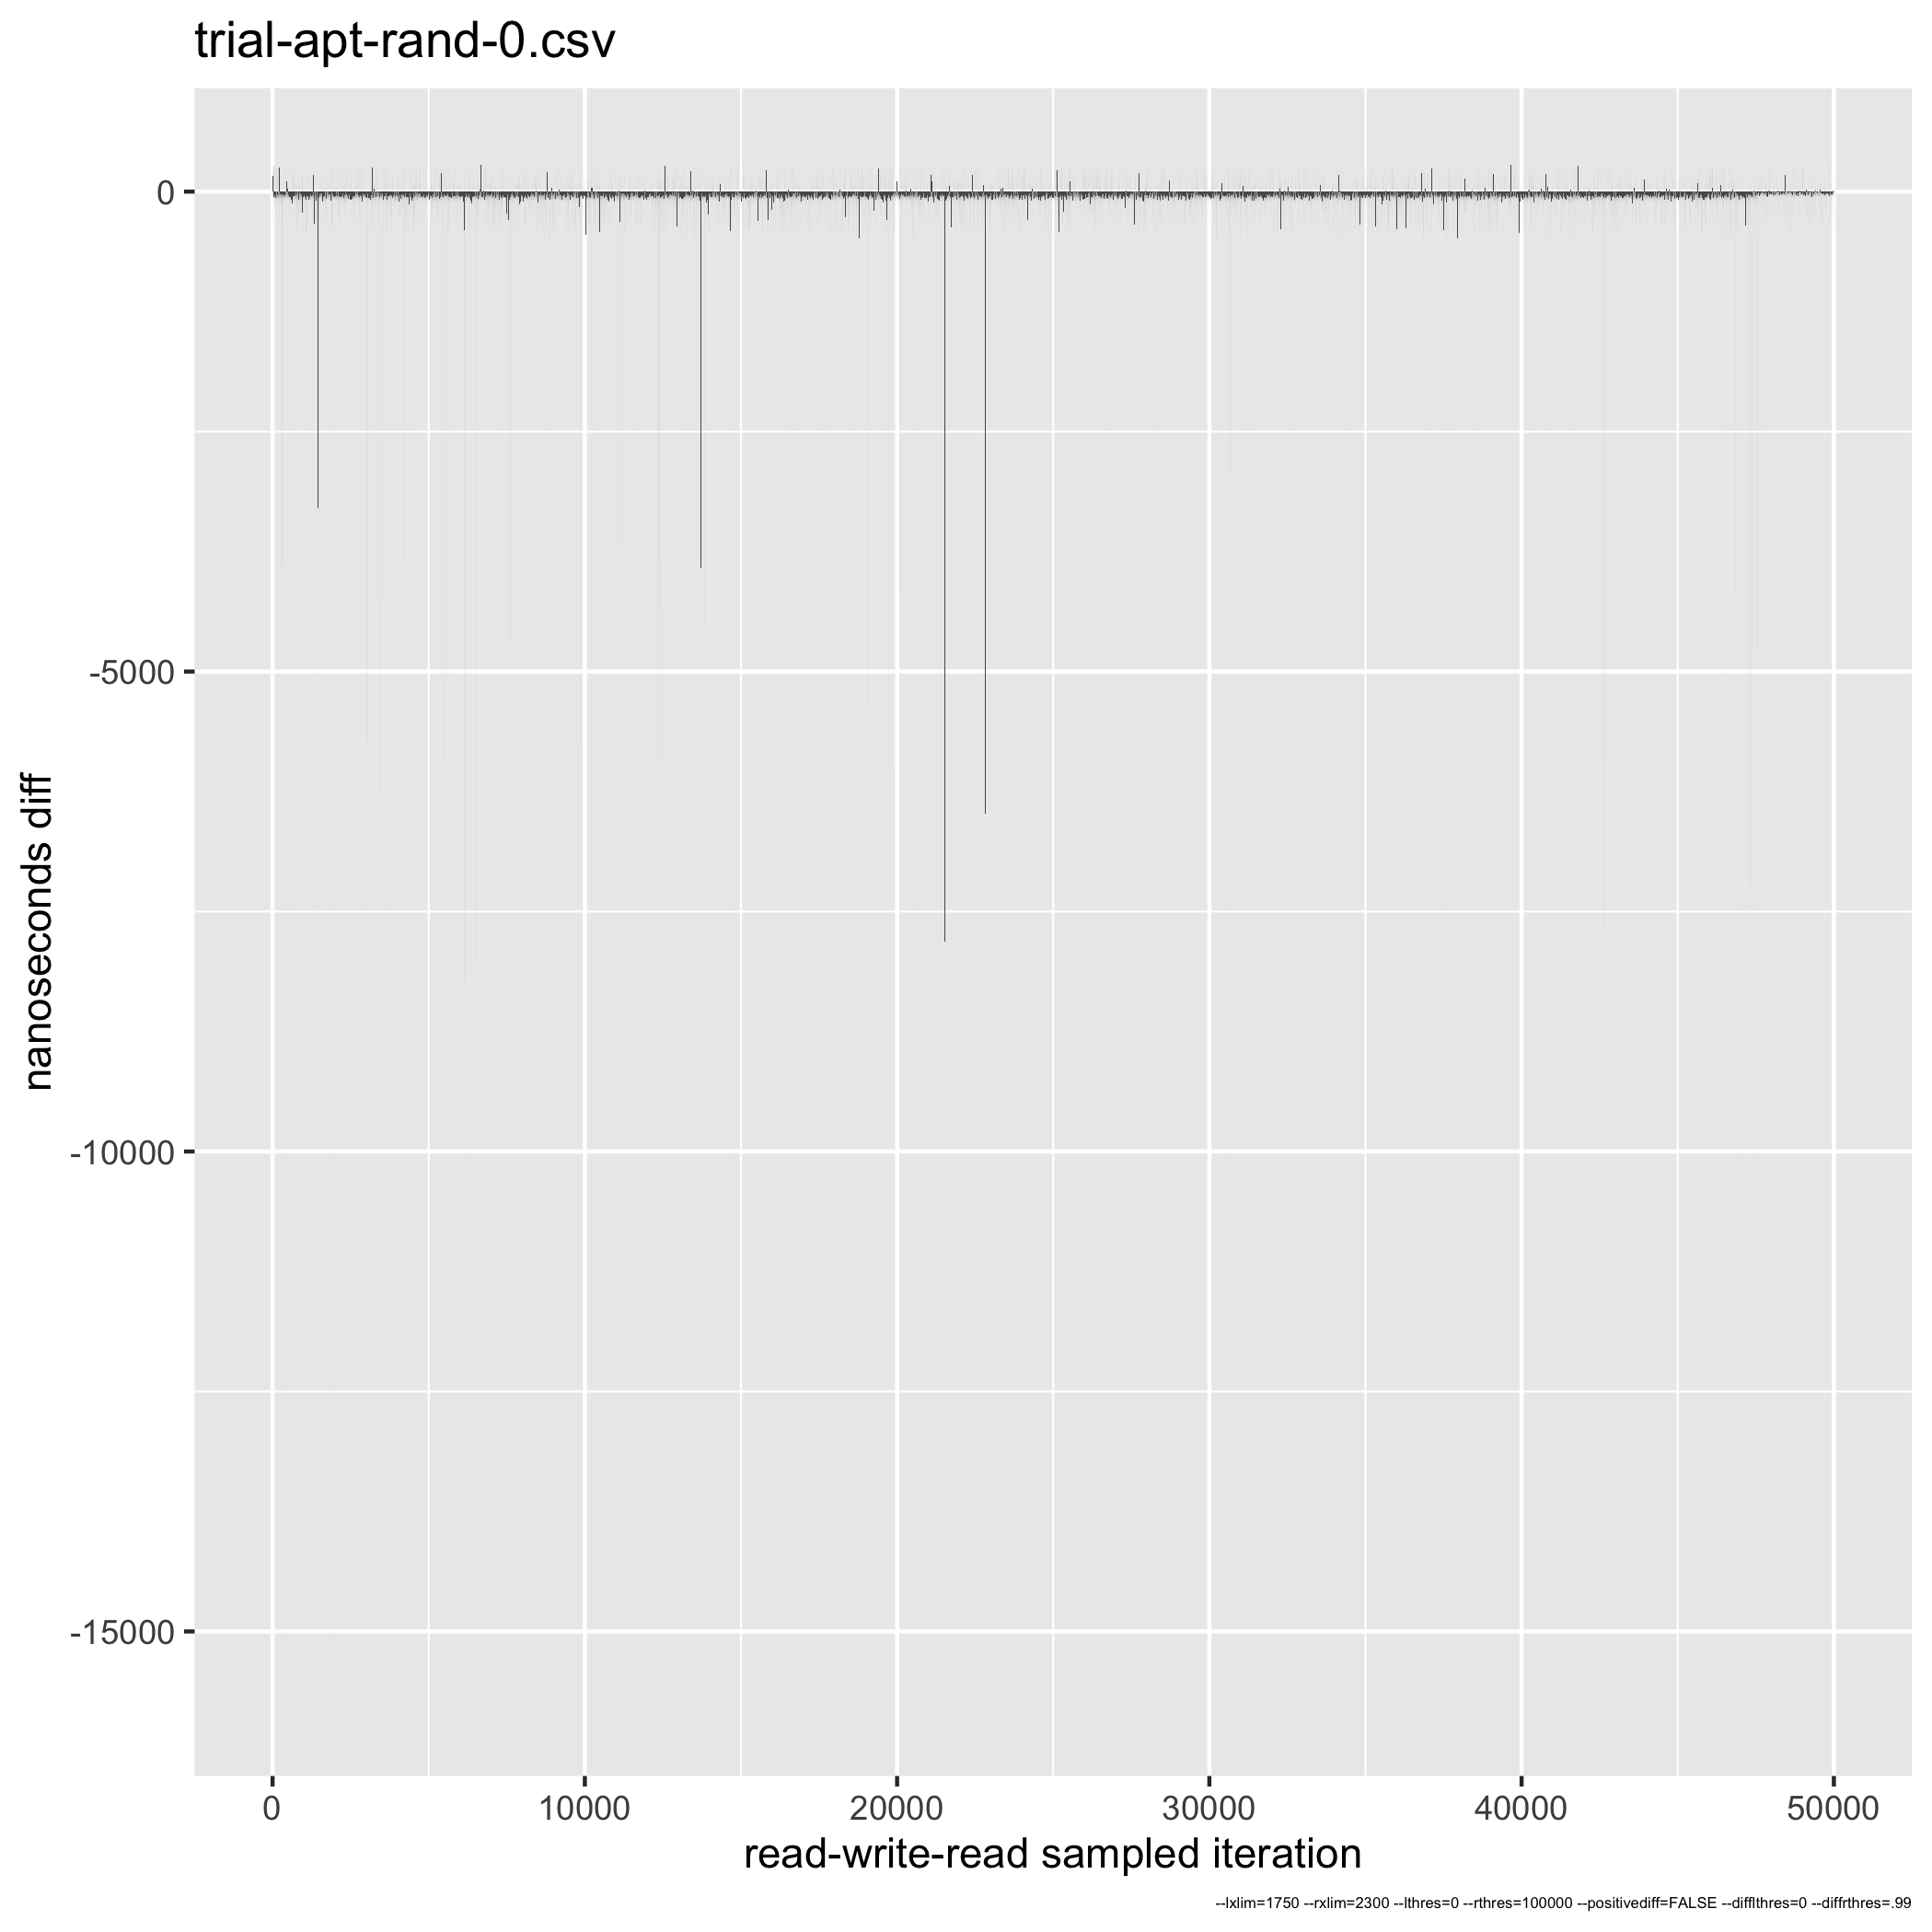
\includegraphics[width=\linewidth]{trial-apt-rand-0-barchart.png}

  \end{column}

 \end{columns}
\end{frame}

\begin{frame}
 \frametitle{Sequential Access Method}
 Tended to consistently produce the results we wanted but the data was noisier.
 \begin{columns}
  \begin{column}{0.5\textwidth}
   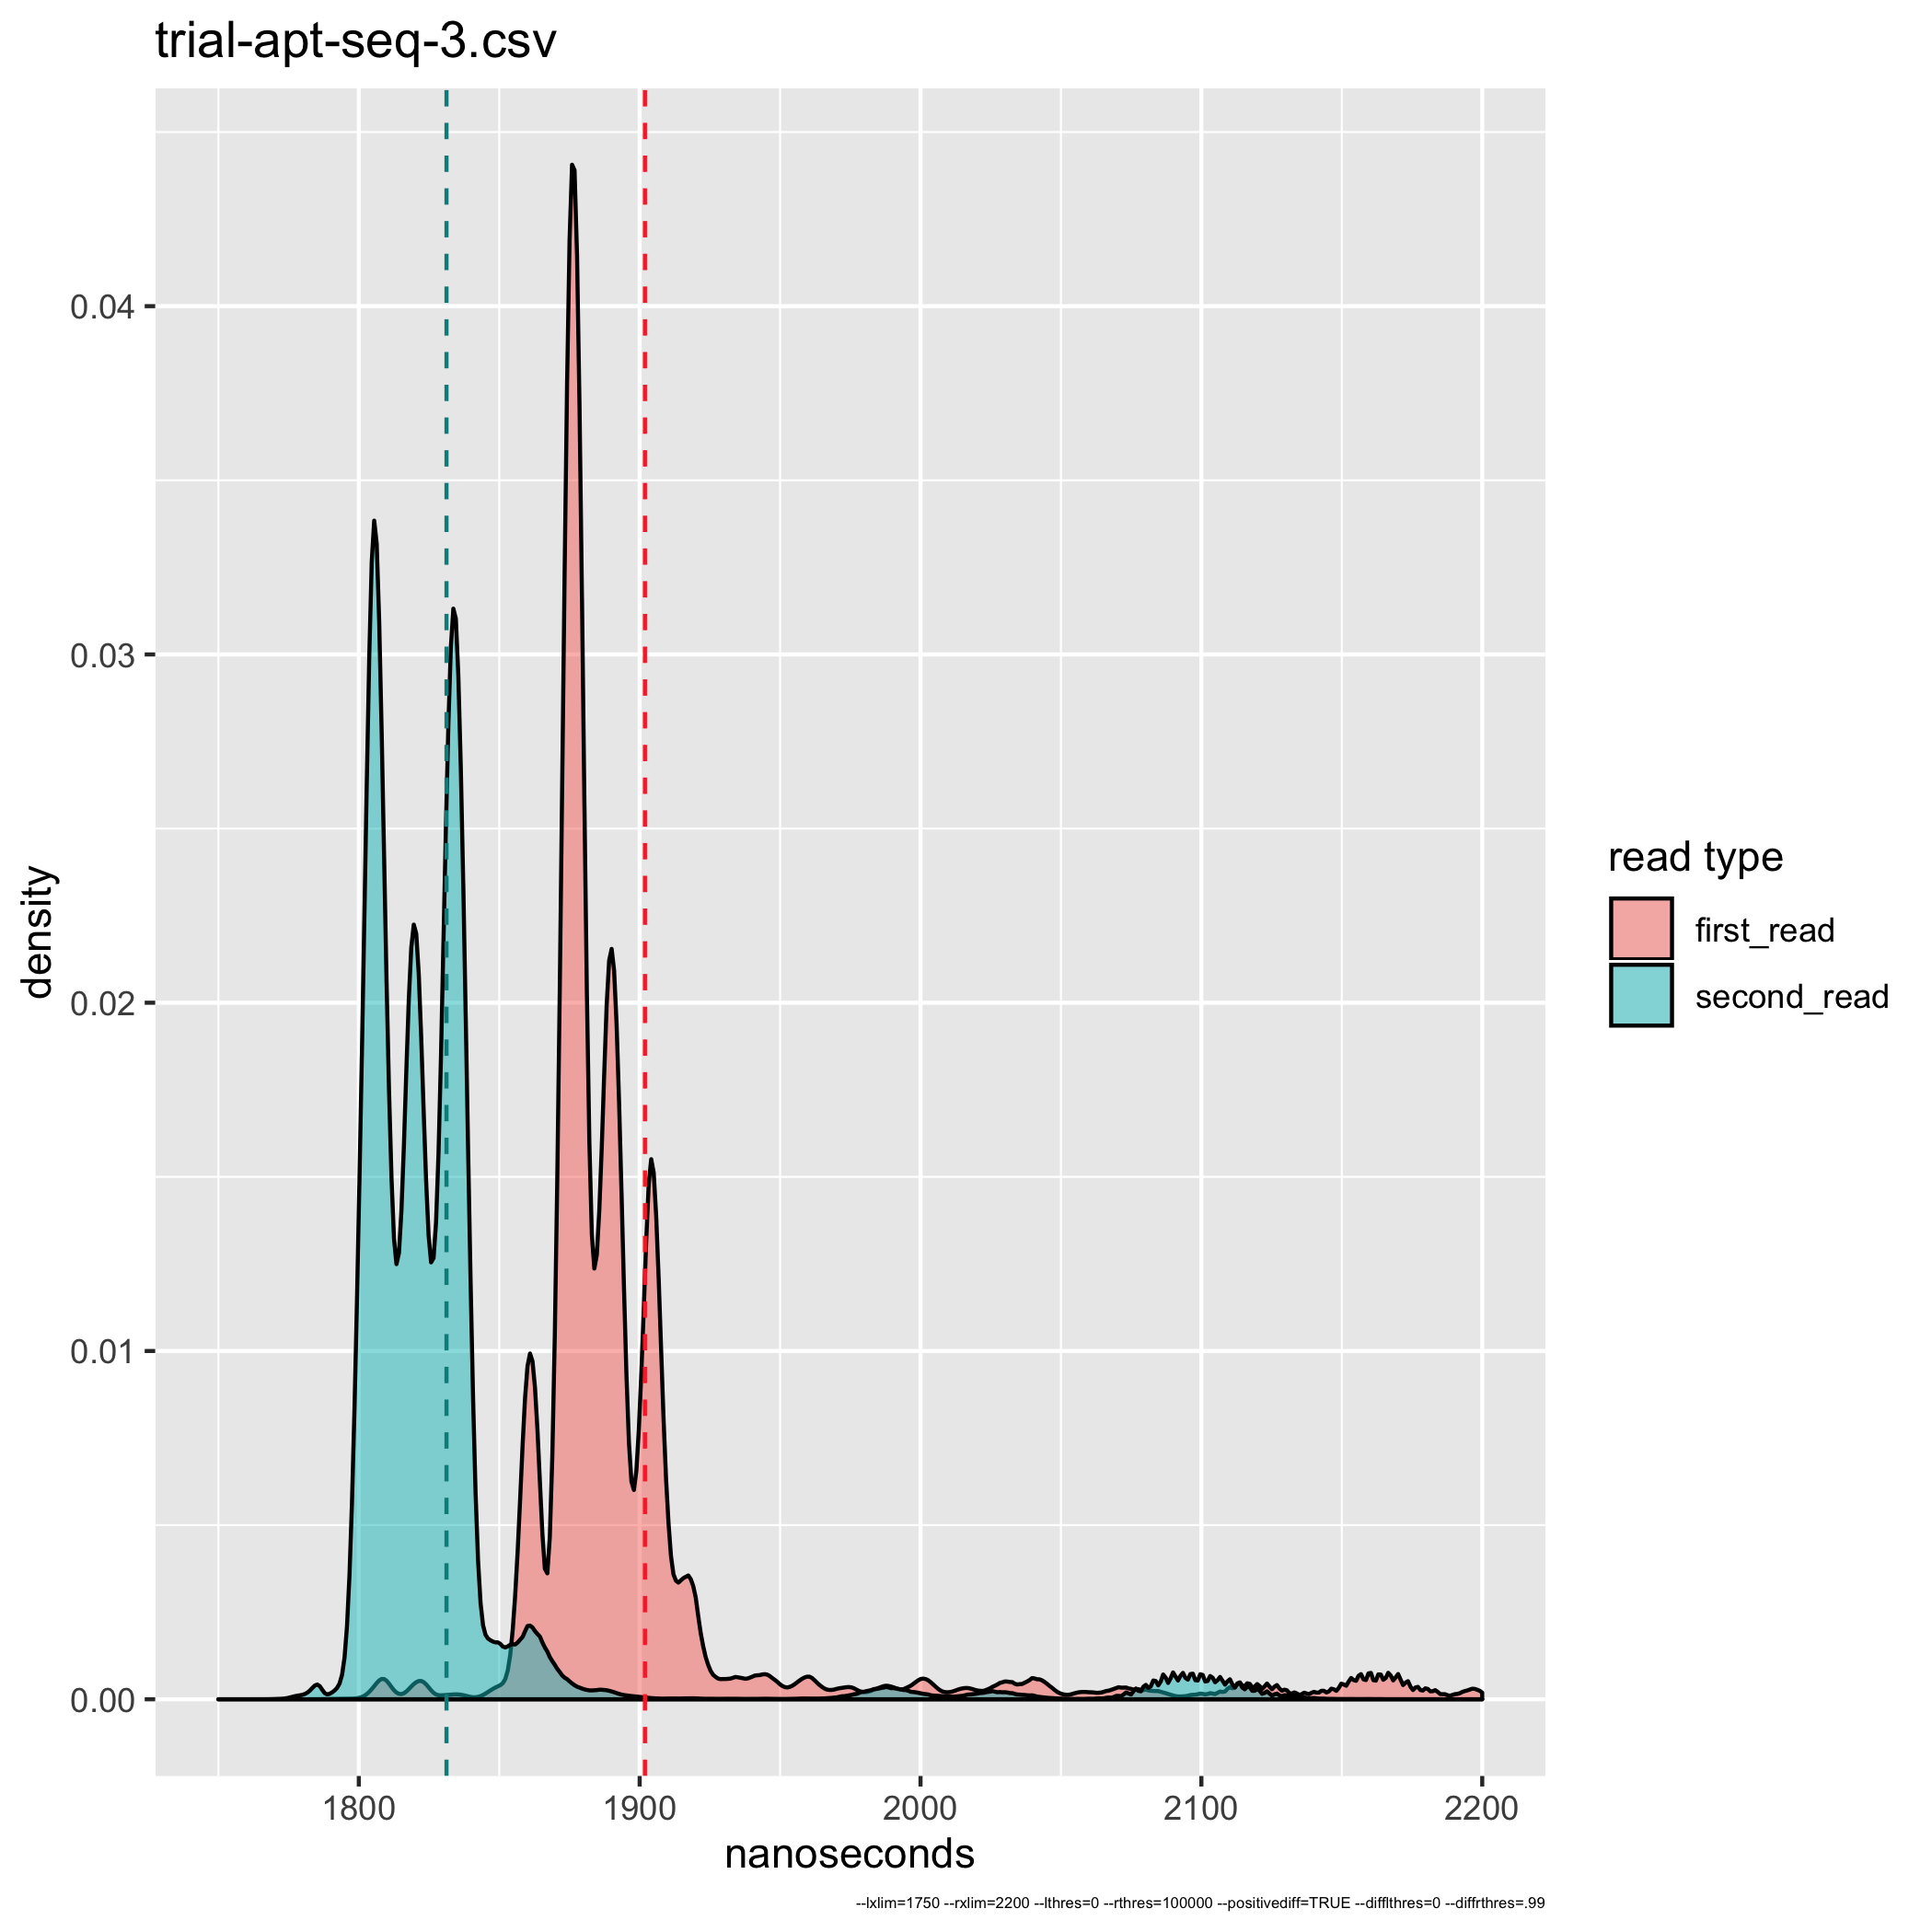
\includegraphics[width=\linewidth]{trial-apt-seq-3-histogram.png}

  \end{column}
  \begin{column}{0.5\textwidth}
   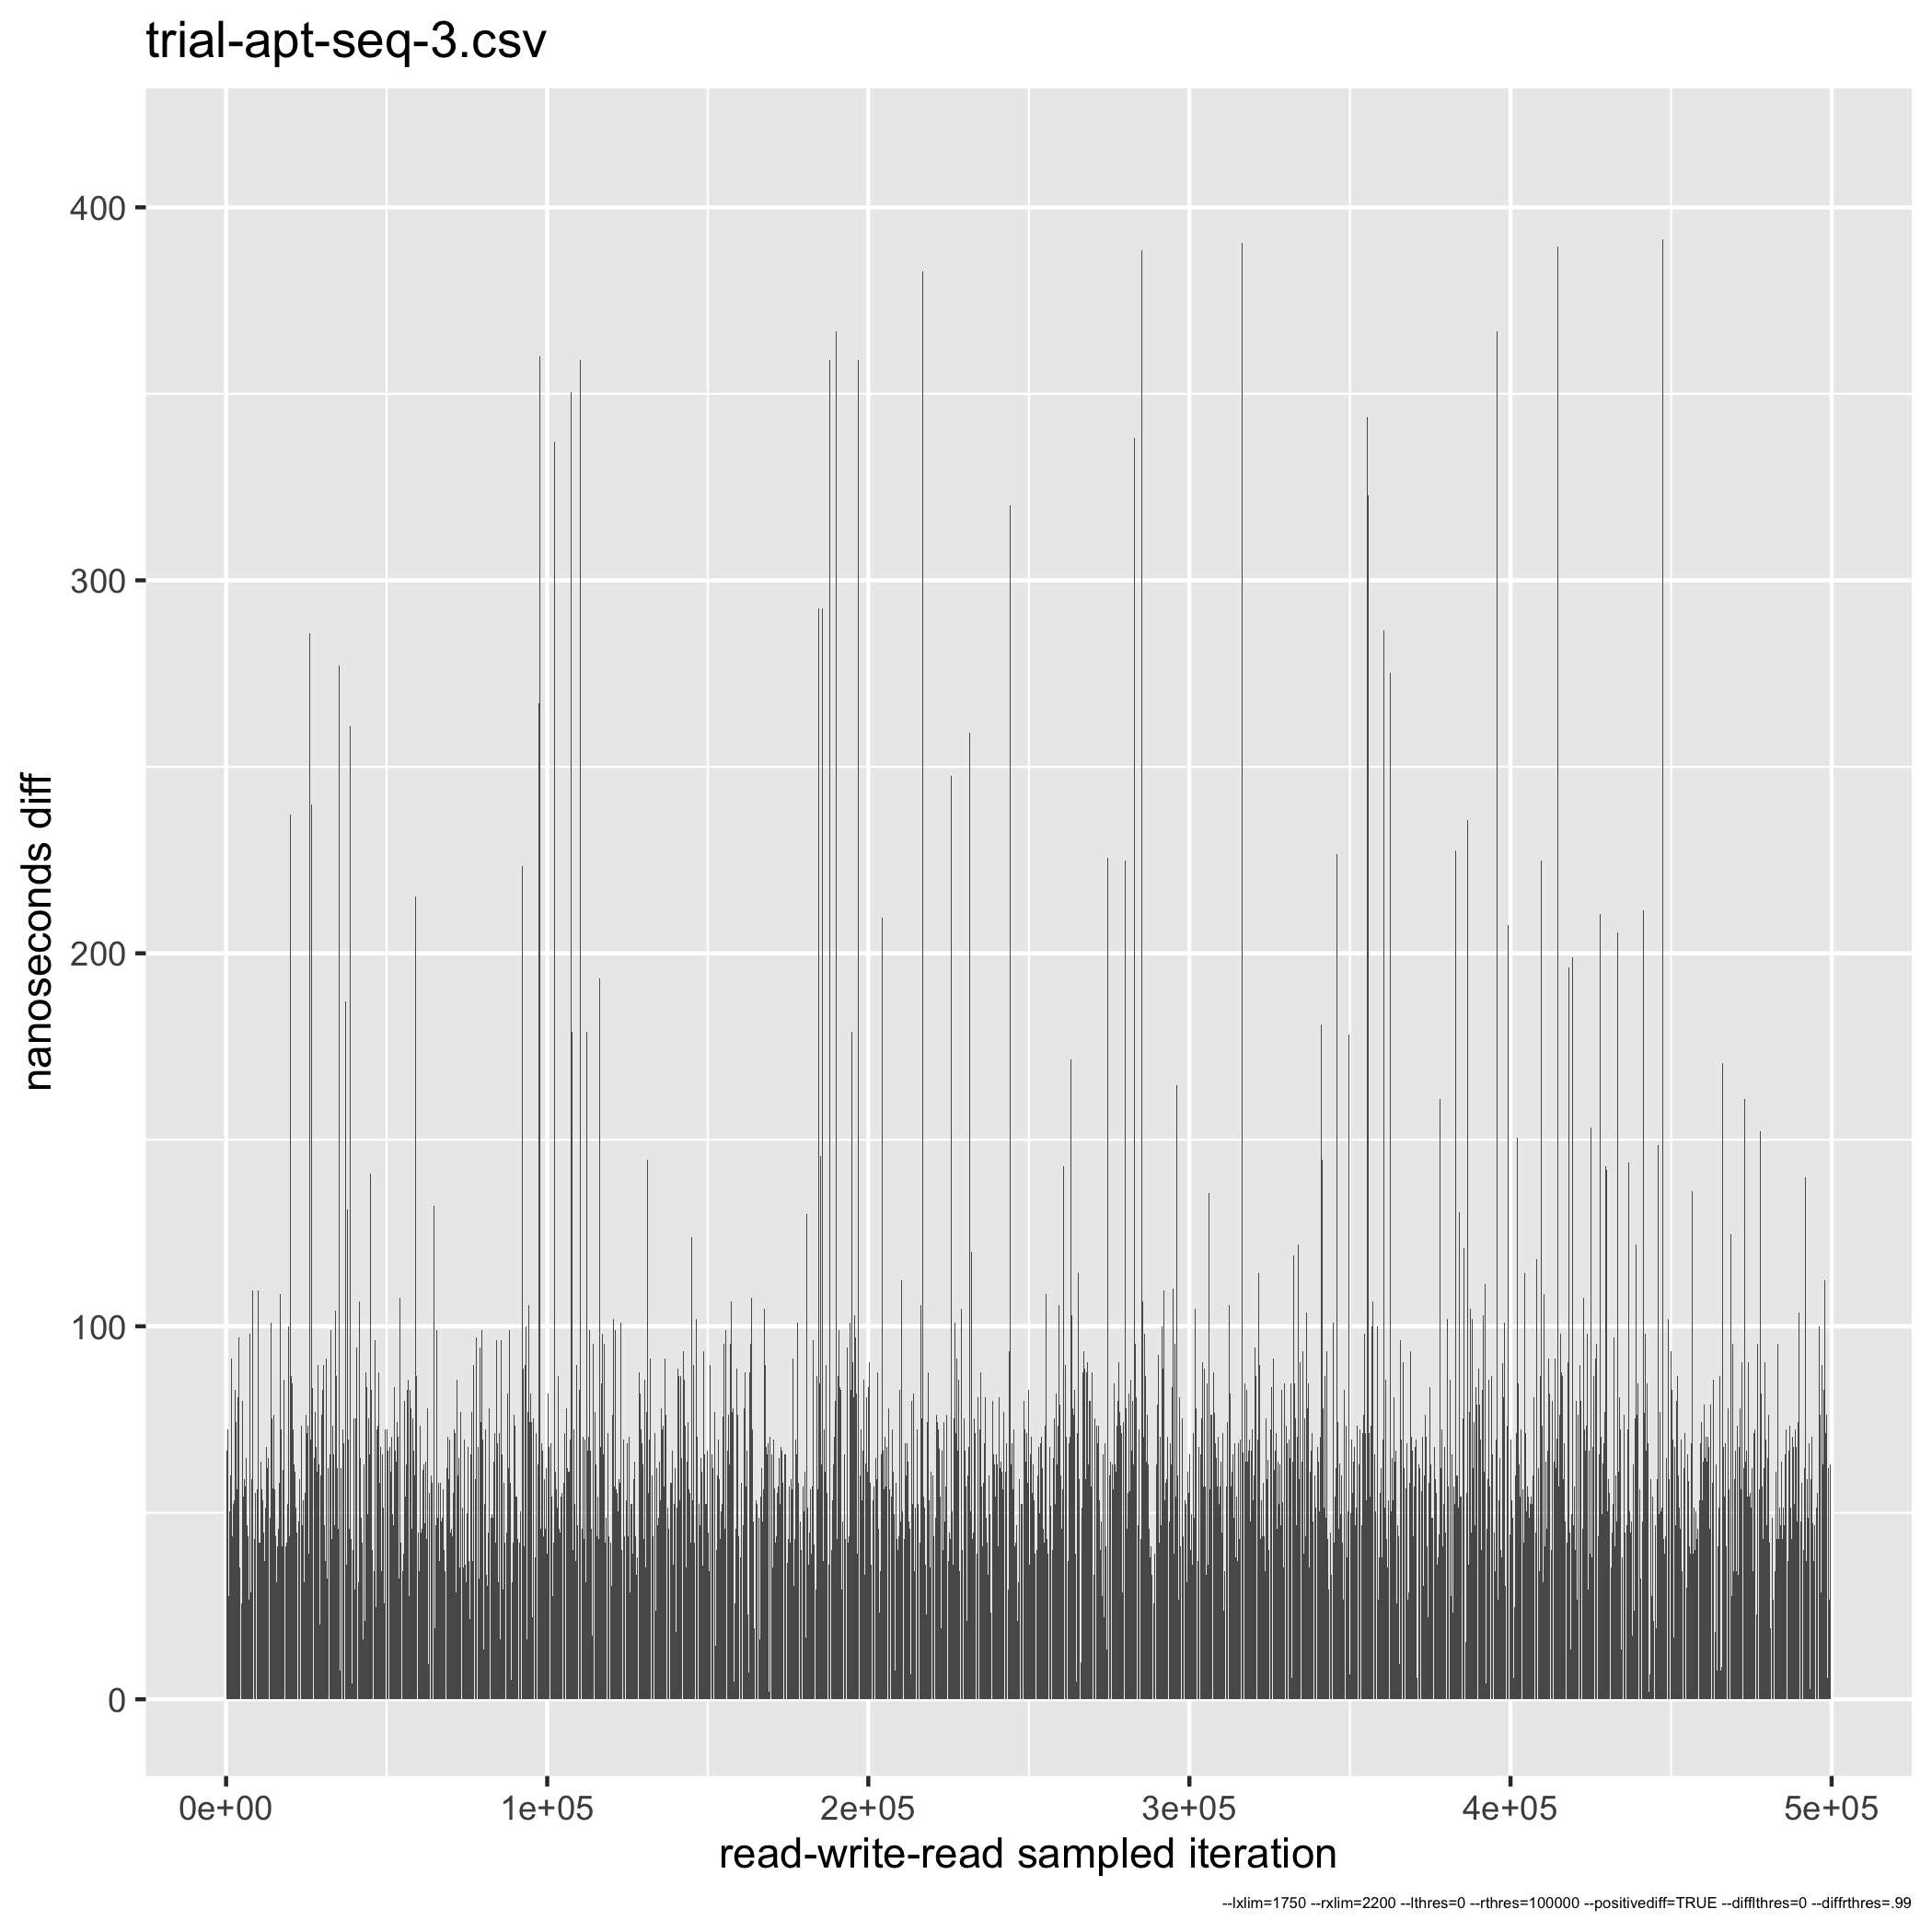
\includegraphics[width=\linewidth]{trial-apt-seq-3-barchart.png}

  \end{column}

 \end{columns}
\end{frame}

\begin{frame}
 \frametitle{Sequential Access Method}
 \begin{columns}
  \begin{column}{0.5\textwidth}
   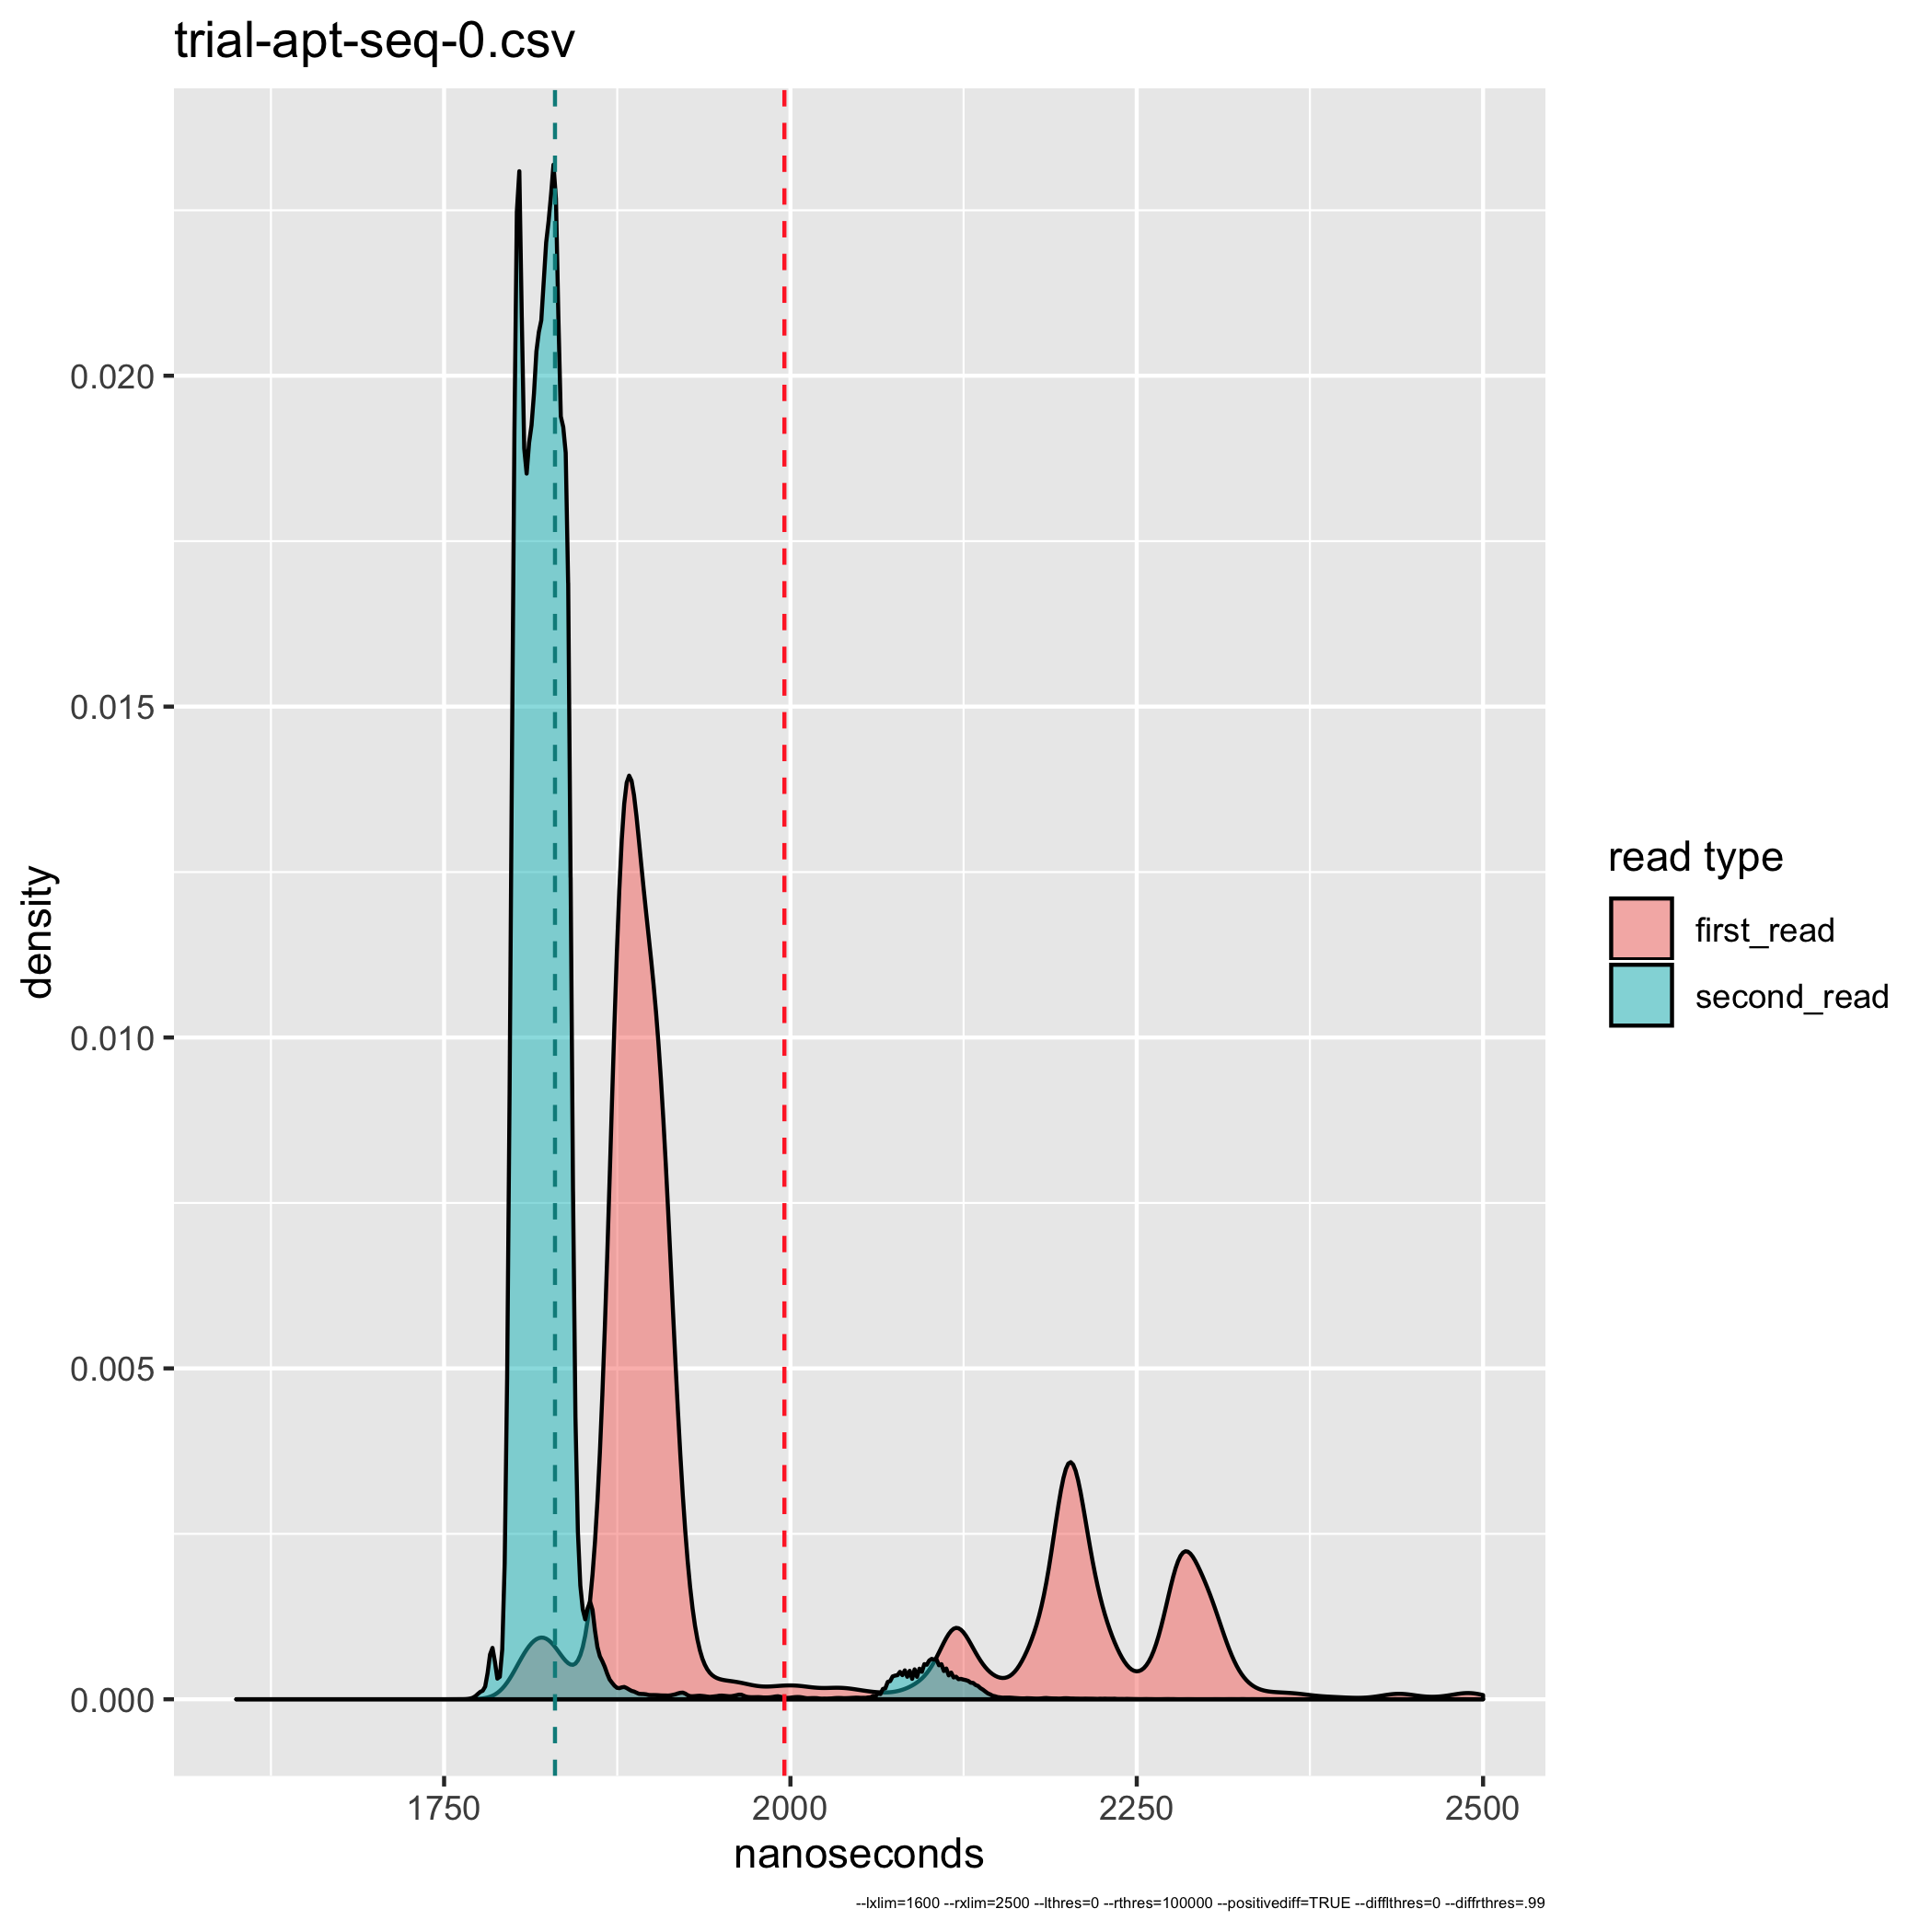
\includegraphics[width=\linewidth]{trial-apt-seq-0-histogram.png}

  \end{column}
  \begin{column}{0.5\textwidth}
   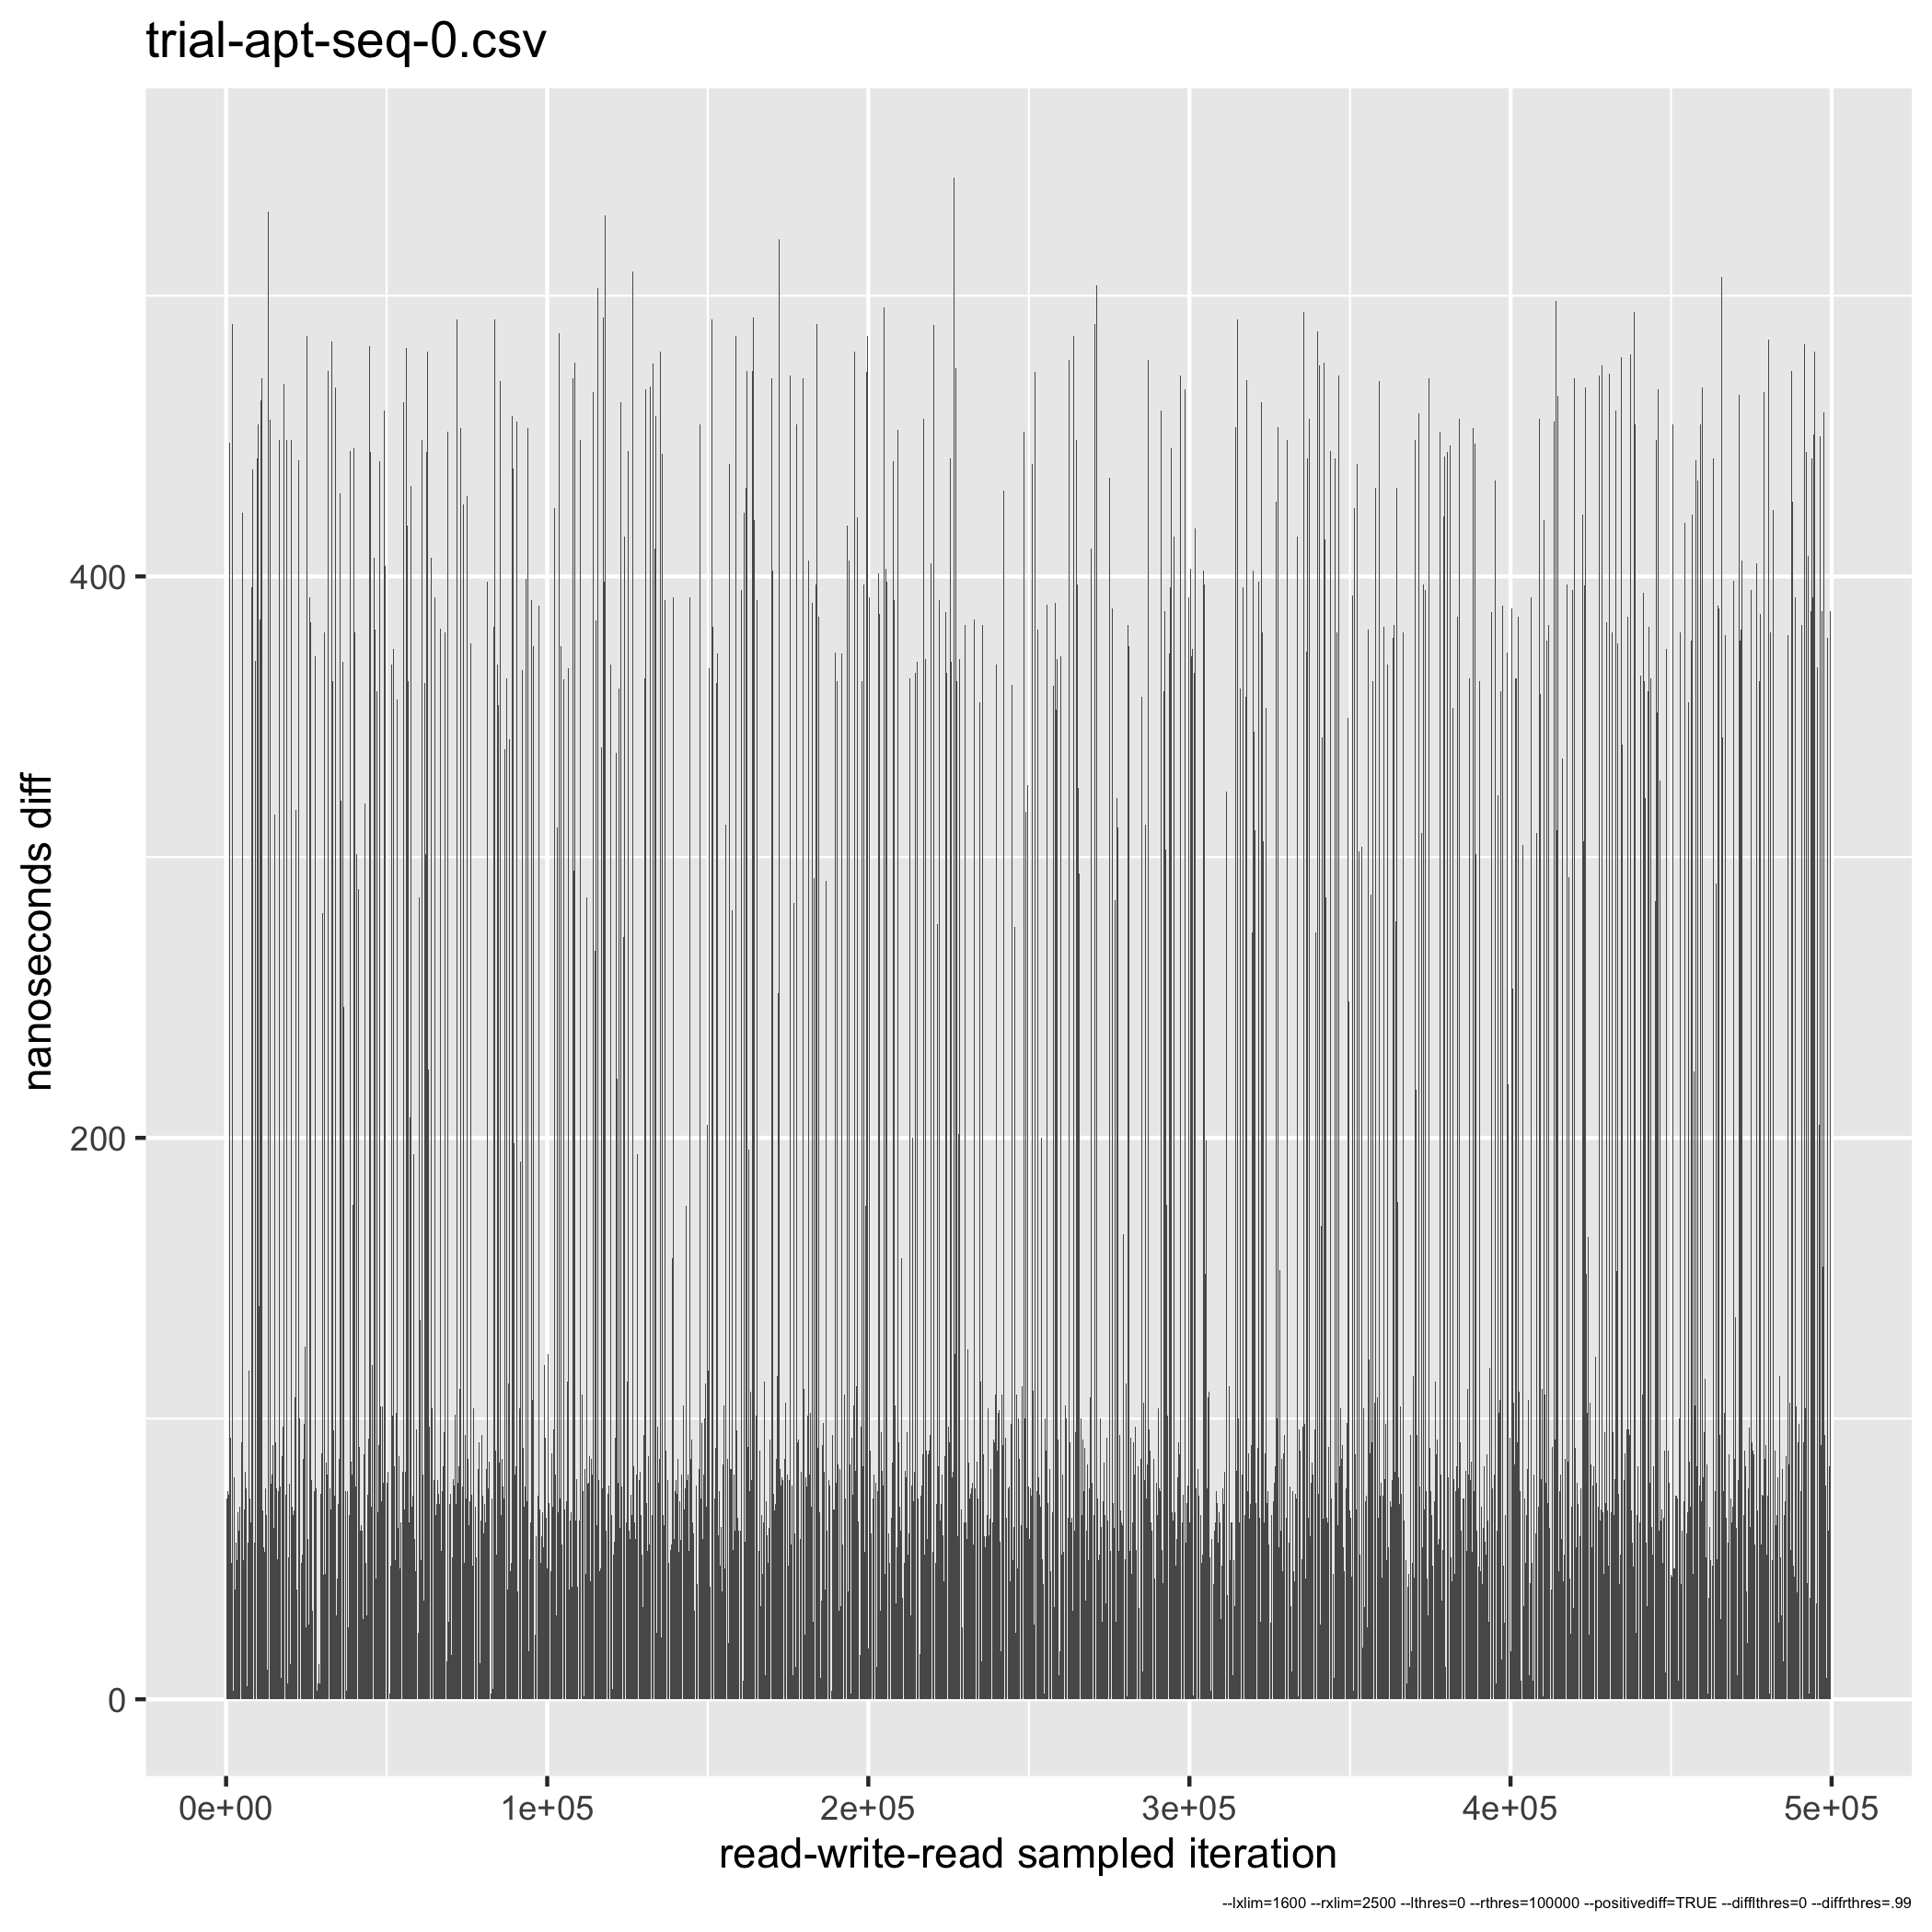
\includegraphics[width=\linewidth]{trial-apt-seq-0-barchart.png}

  \end{column}

 \end{columns}

\end{frame}

\begin{frame}
 \frametitle{Sequential Access Method}
 Sequential access also observed a similar ``diff stepdown'' as \texttt{clflush}.
 \begin{columns}
  \begin{column}{0.5\textwidth}
   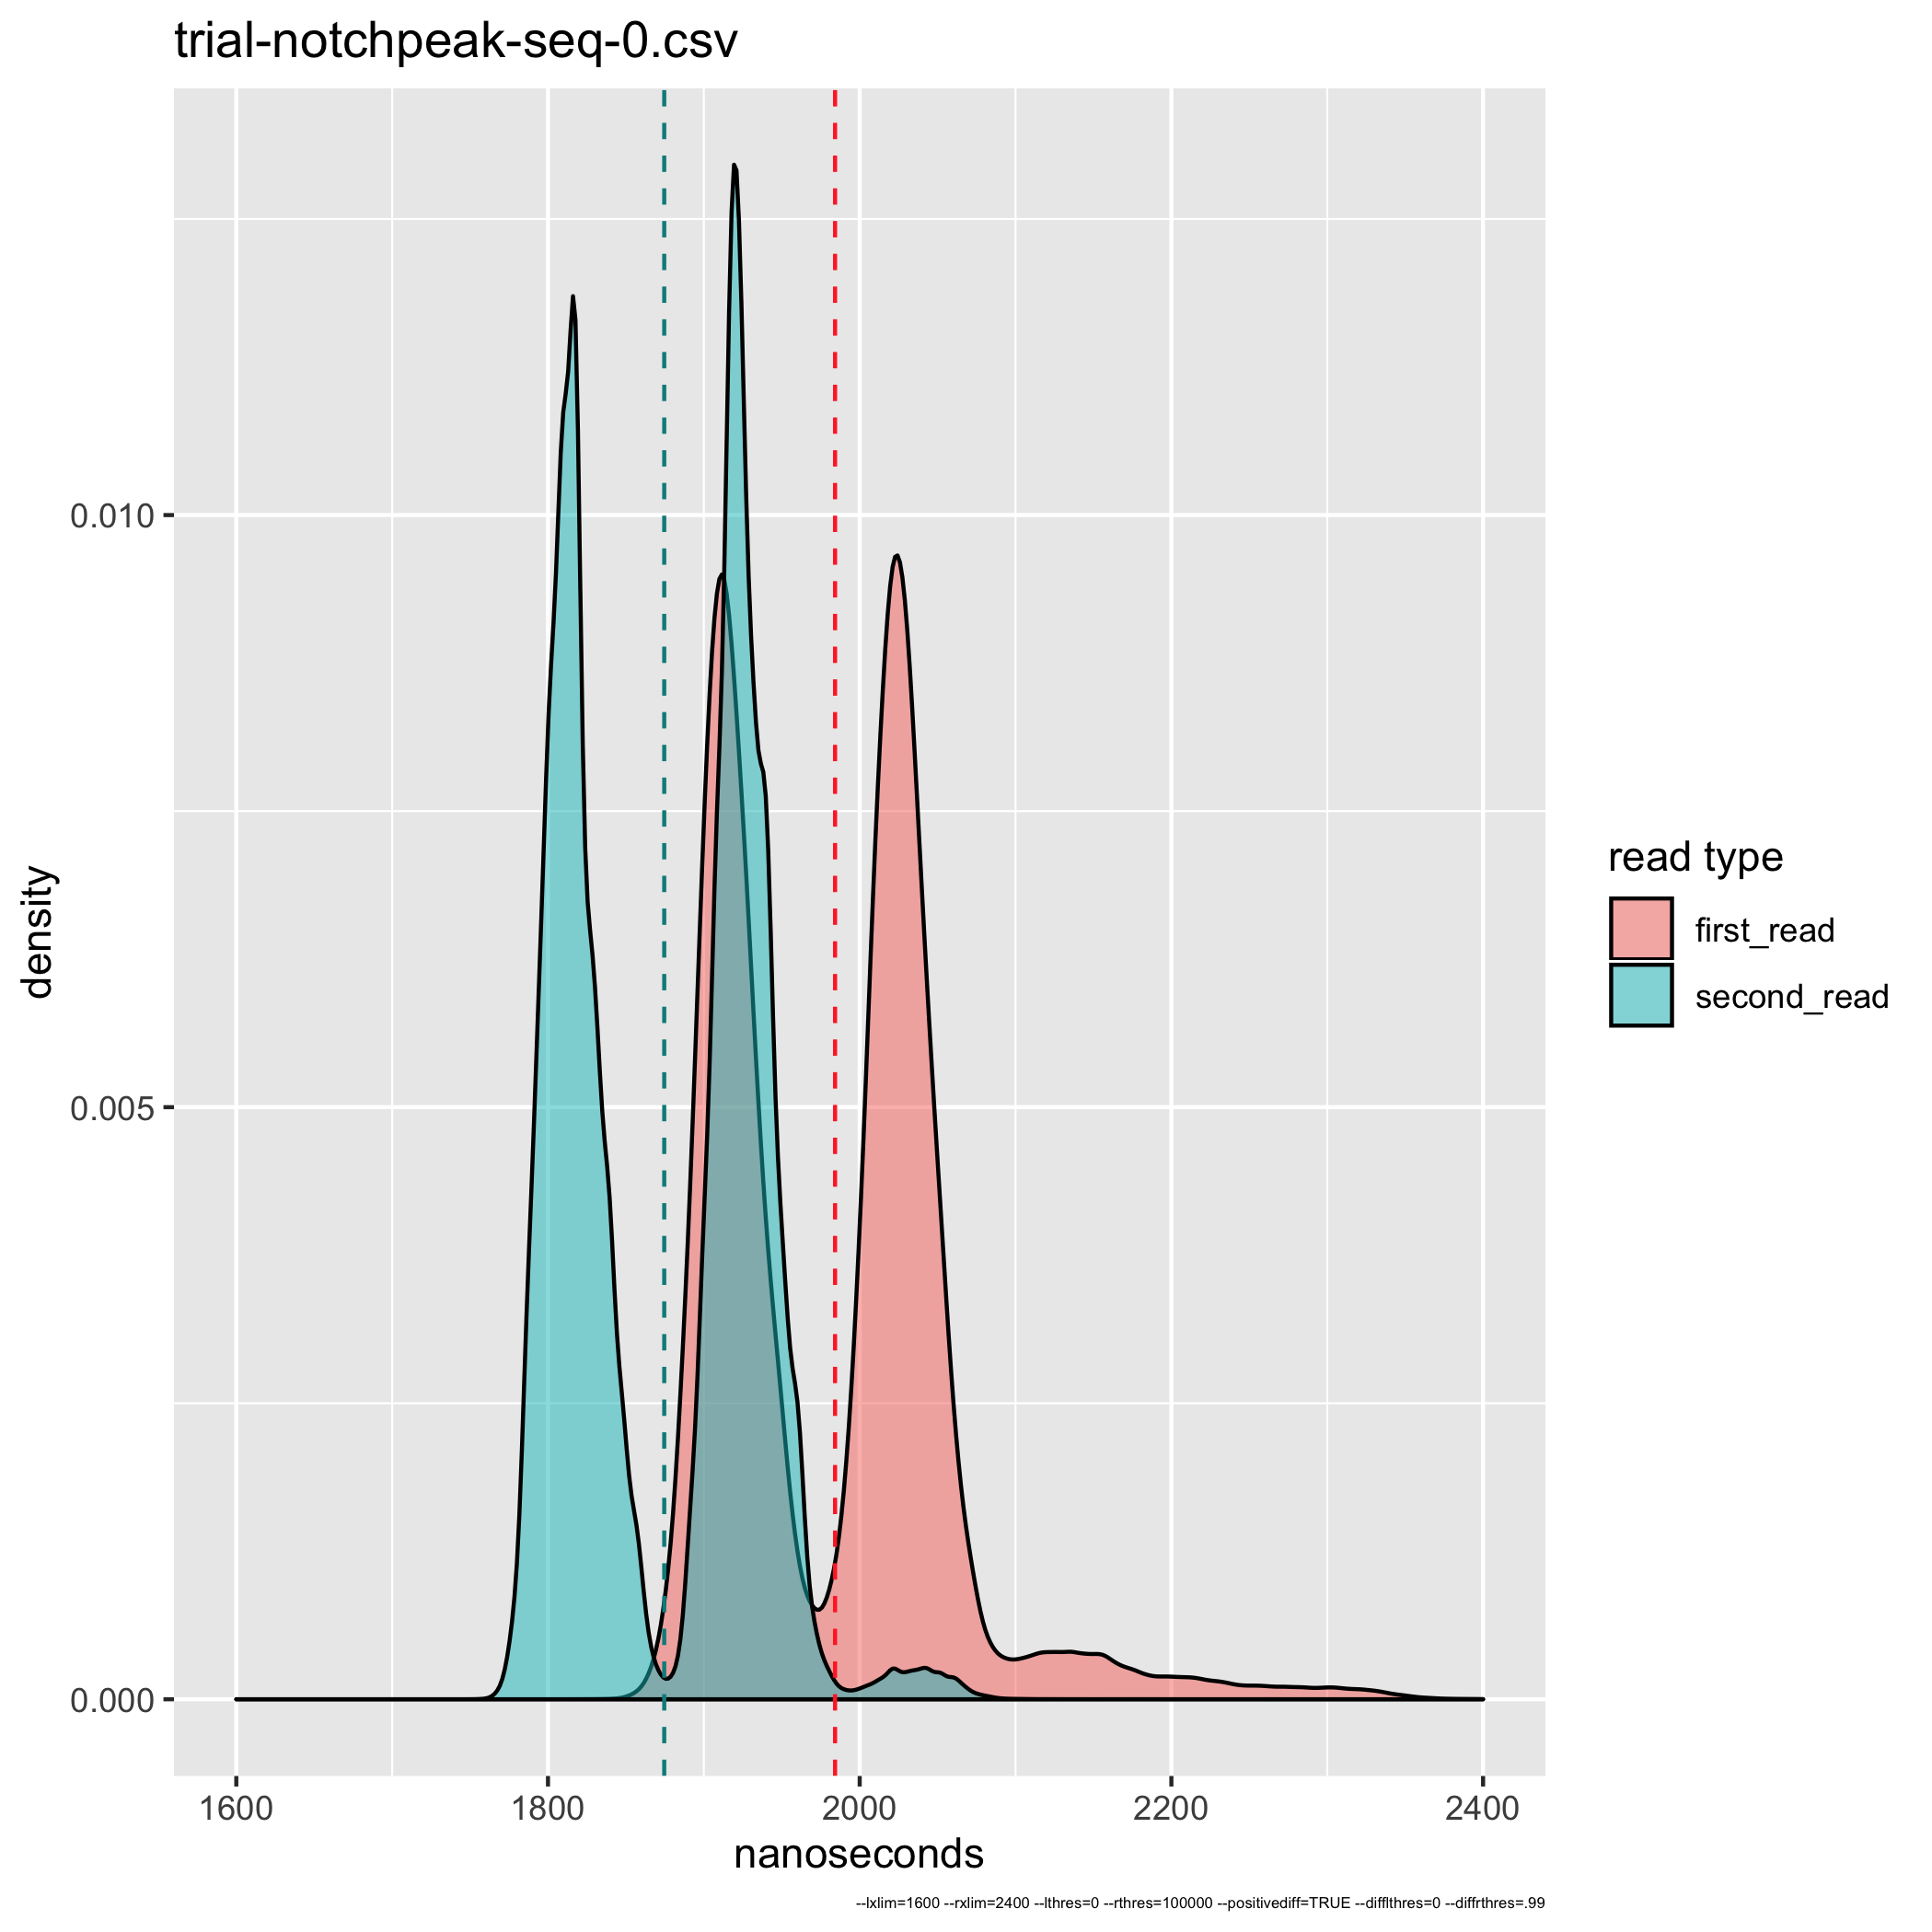
\includegraphics[width=\linewidth]{trial-notchpeak-seq-0-histogram.png}

  \end{column}
  \begin{column}{0.5\textwidth}
   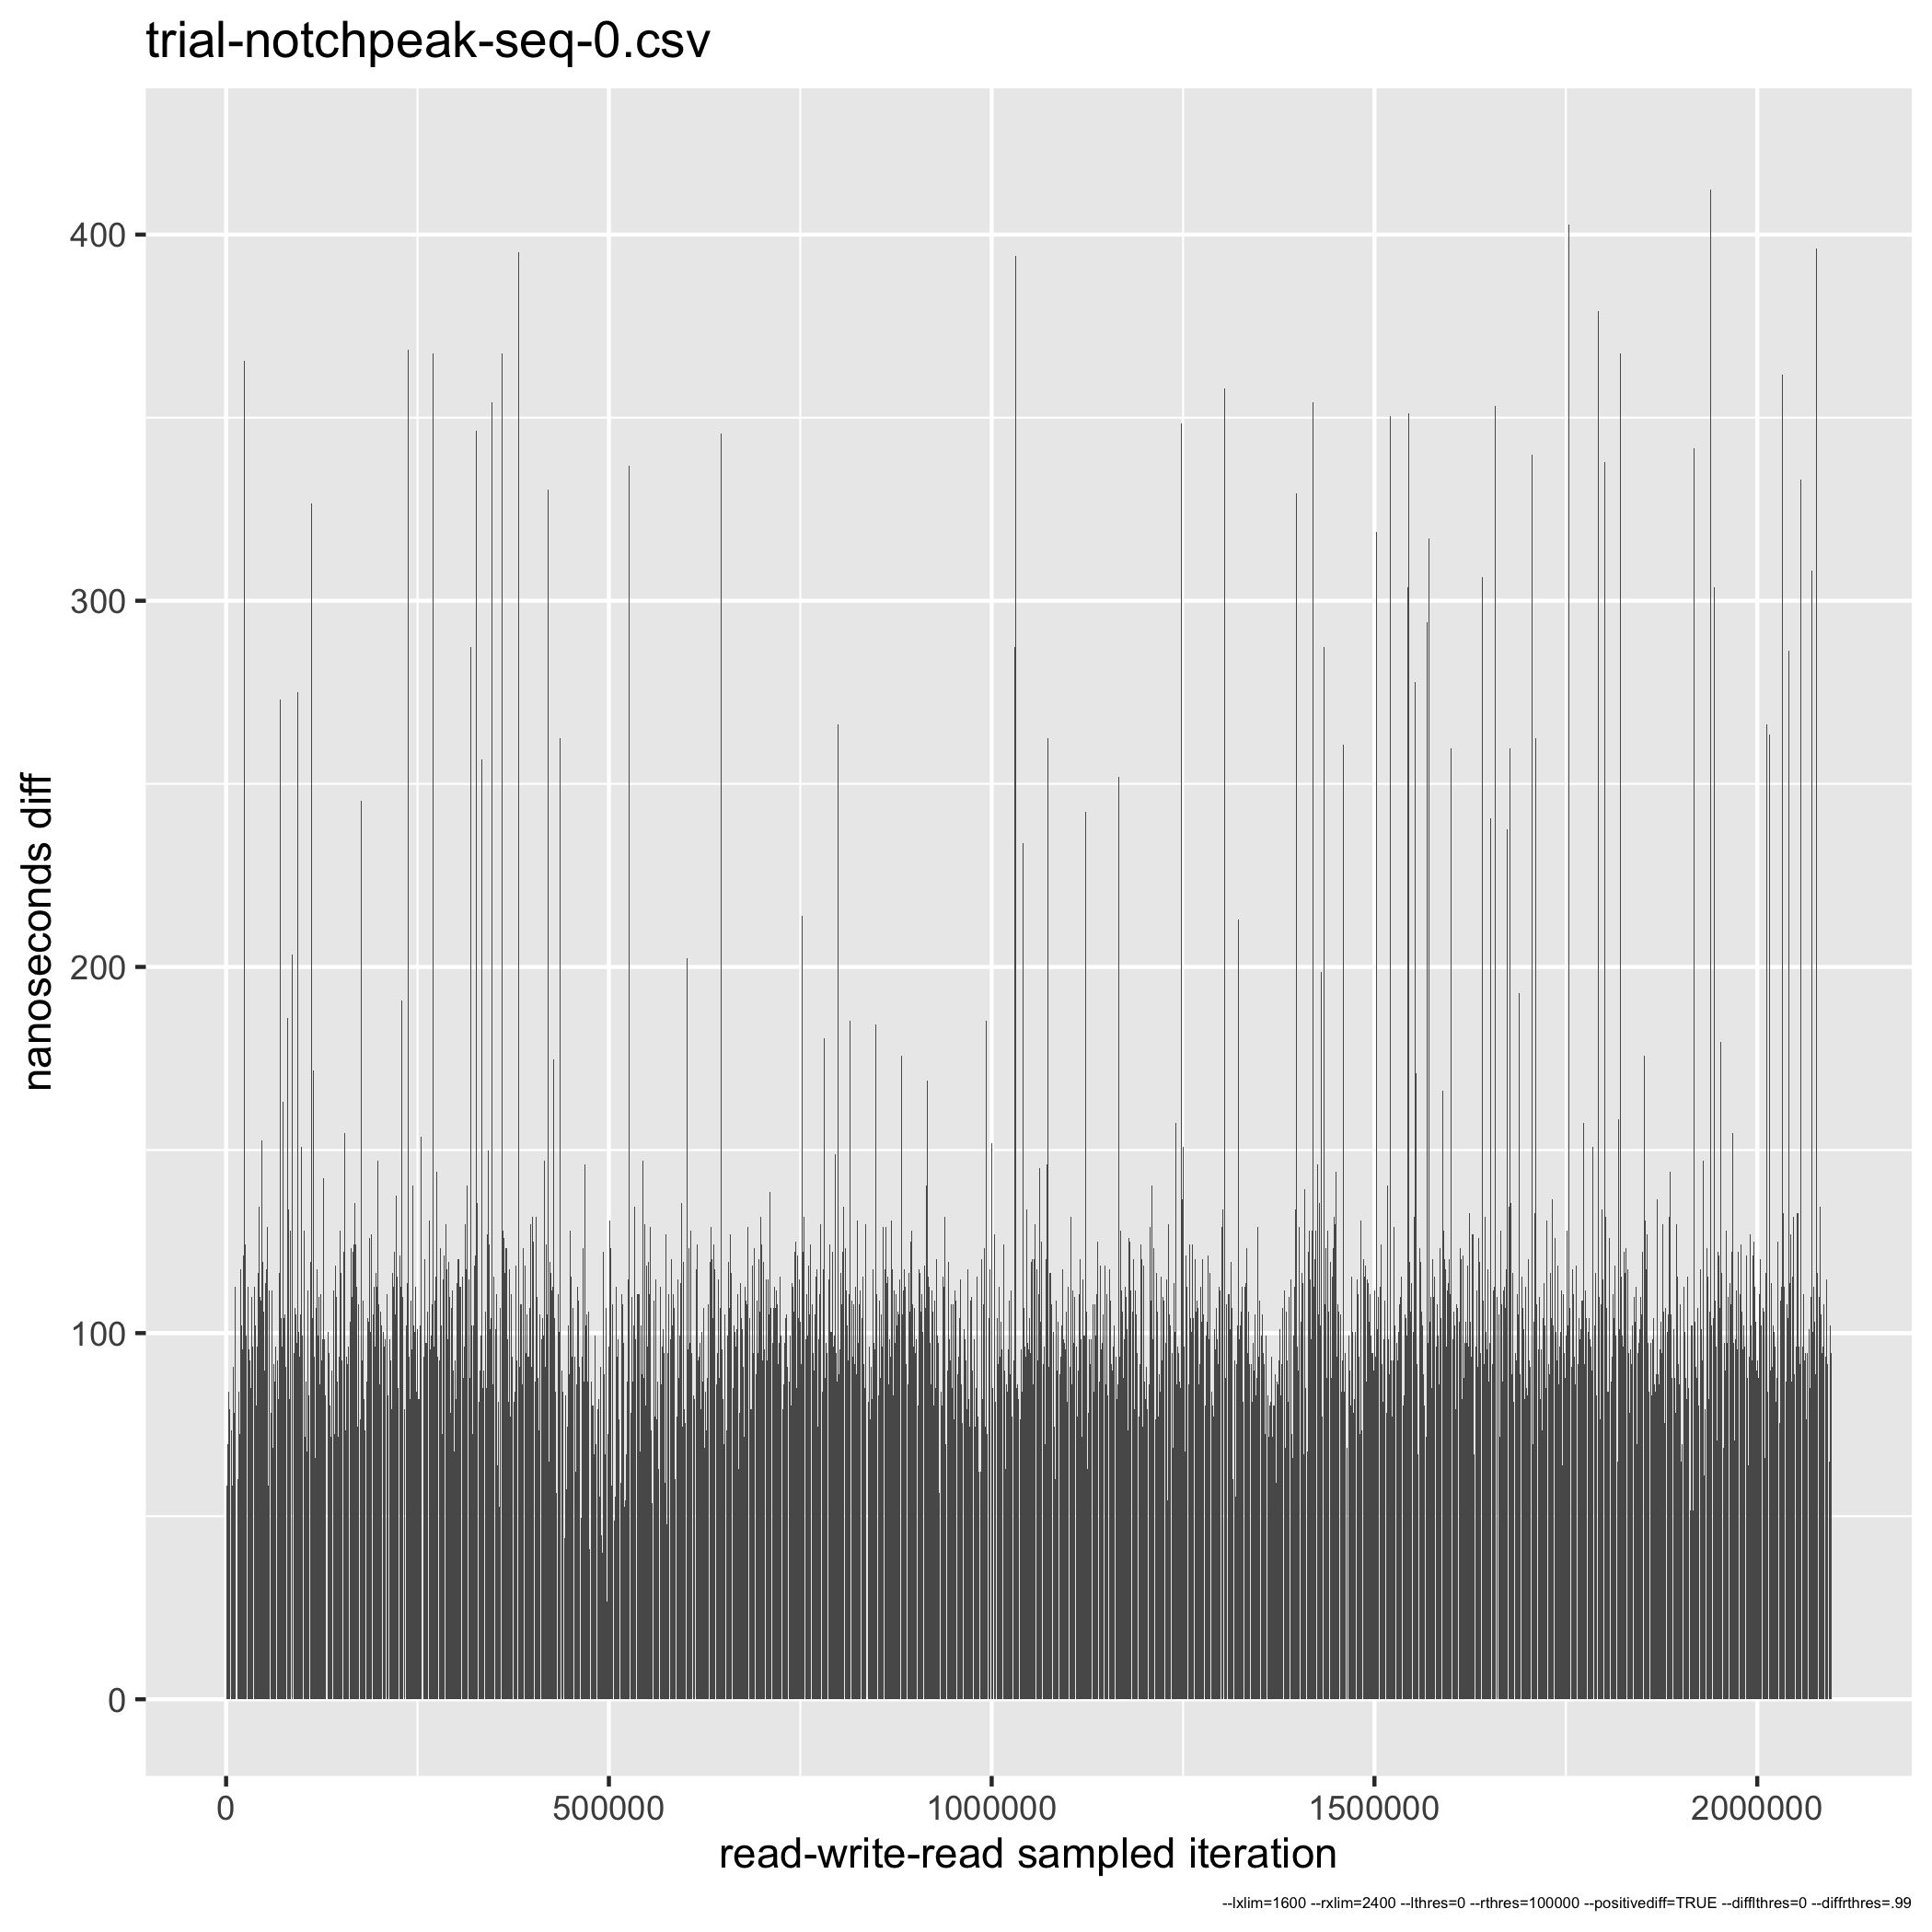
\includegraphics[width=\linewidth]{trial-notchpeak-seq-0-barchart.png}

  \end{column}

 \end{columns}

\end{frame}

\begin{frame}
 \frametitle{Sequential Access Method}
 Sequential access produces expected behavior for read$\rightarrow$read.
 \begin{columns}
  \begin{column}{0.5\textwidth}
   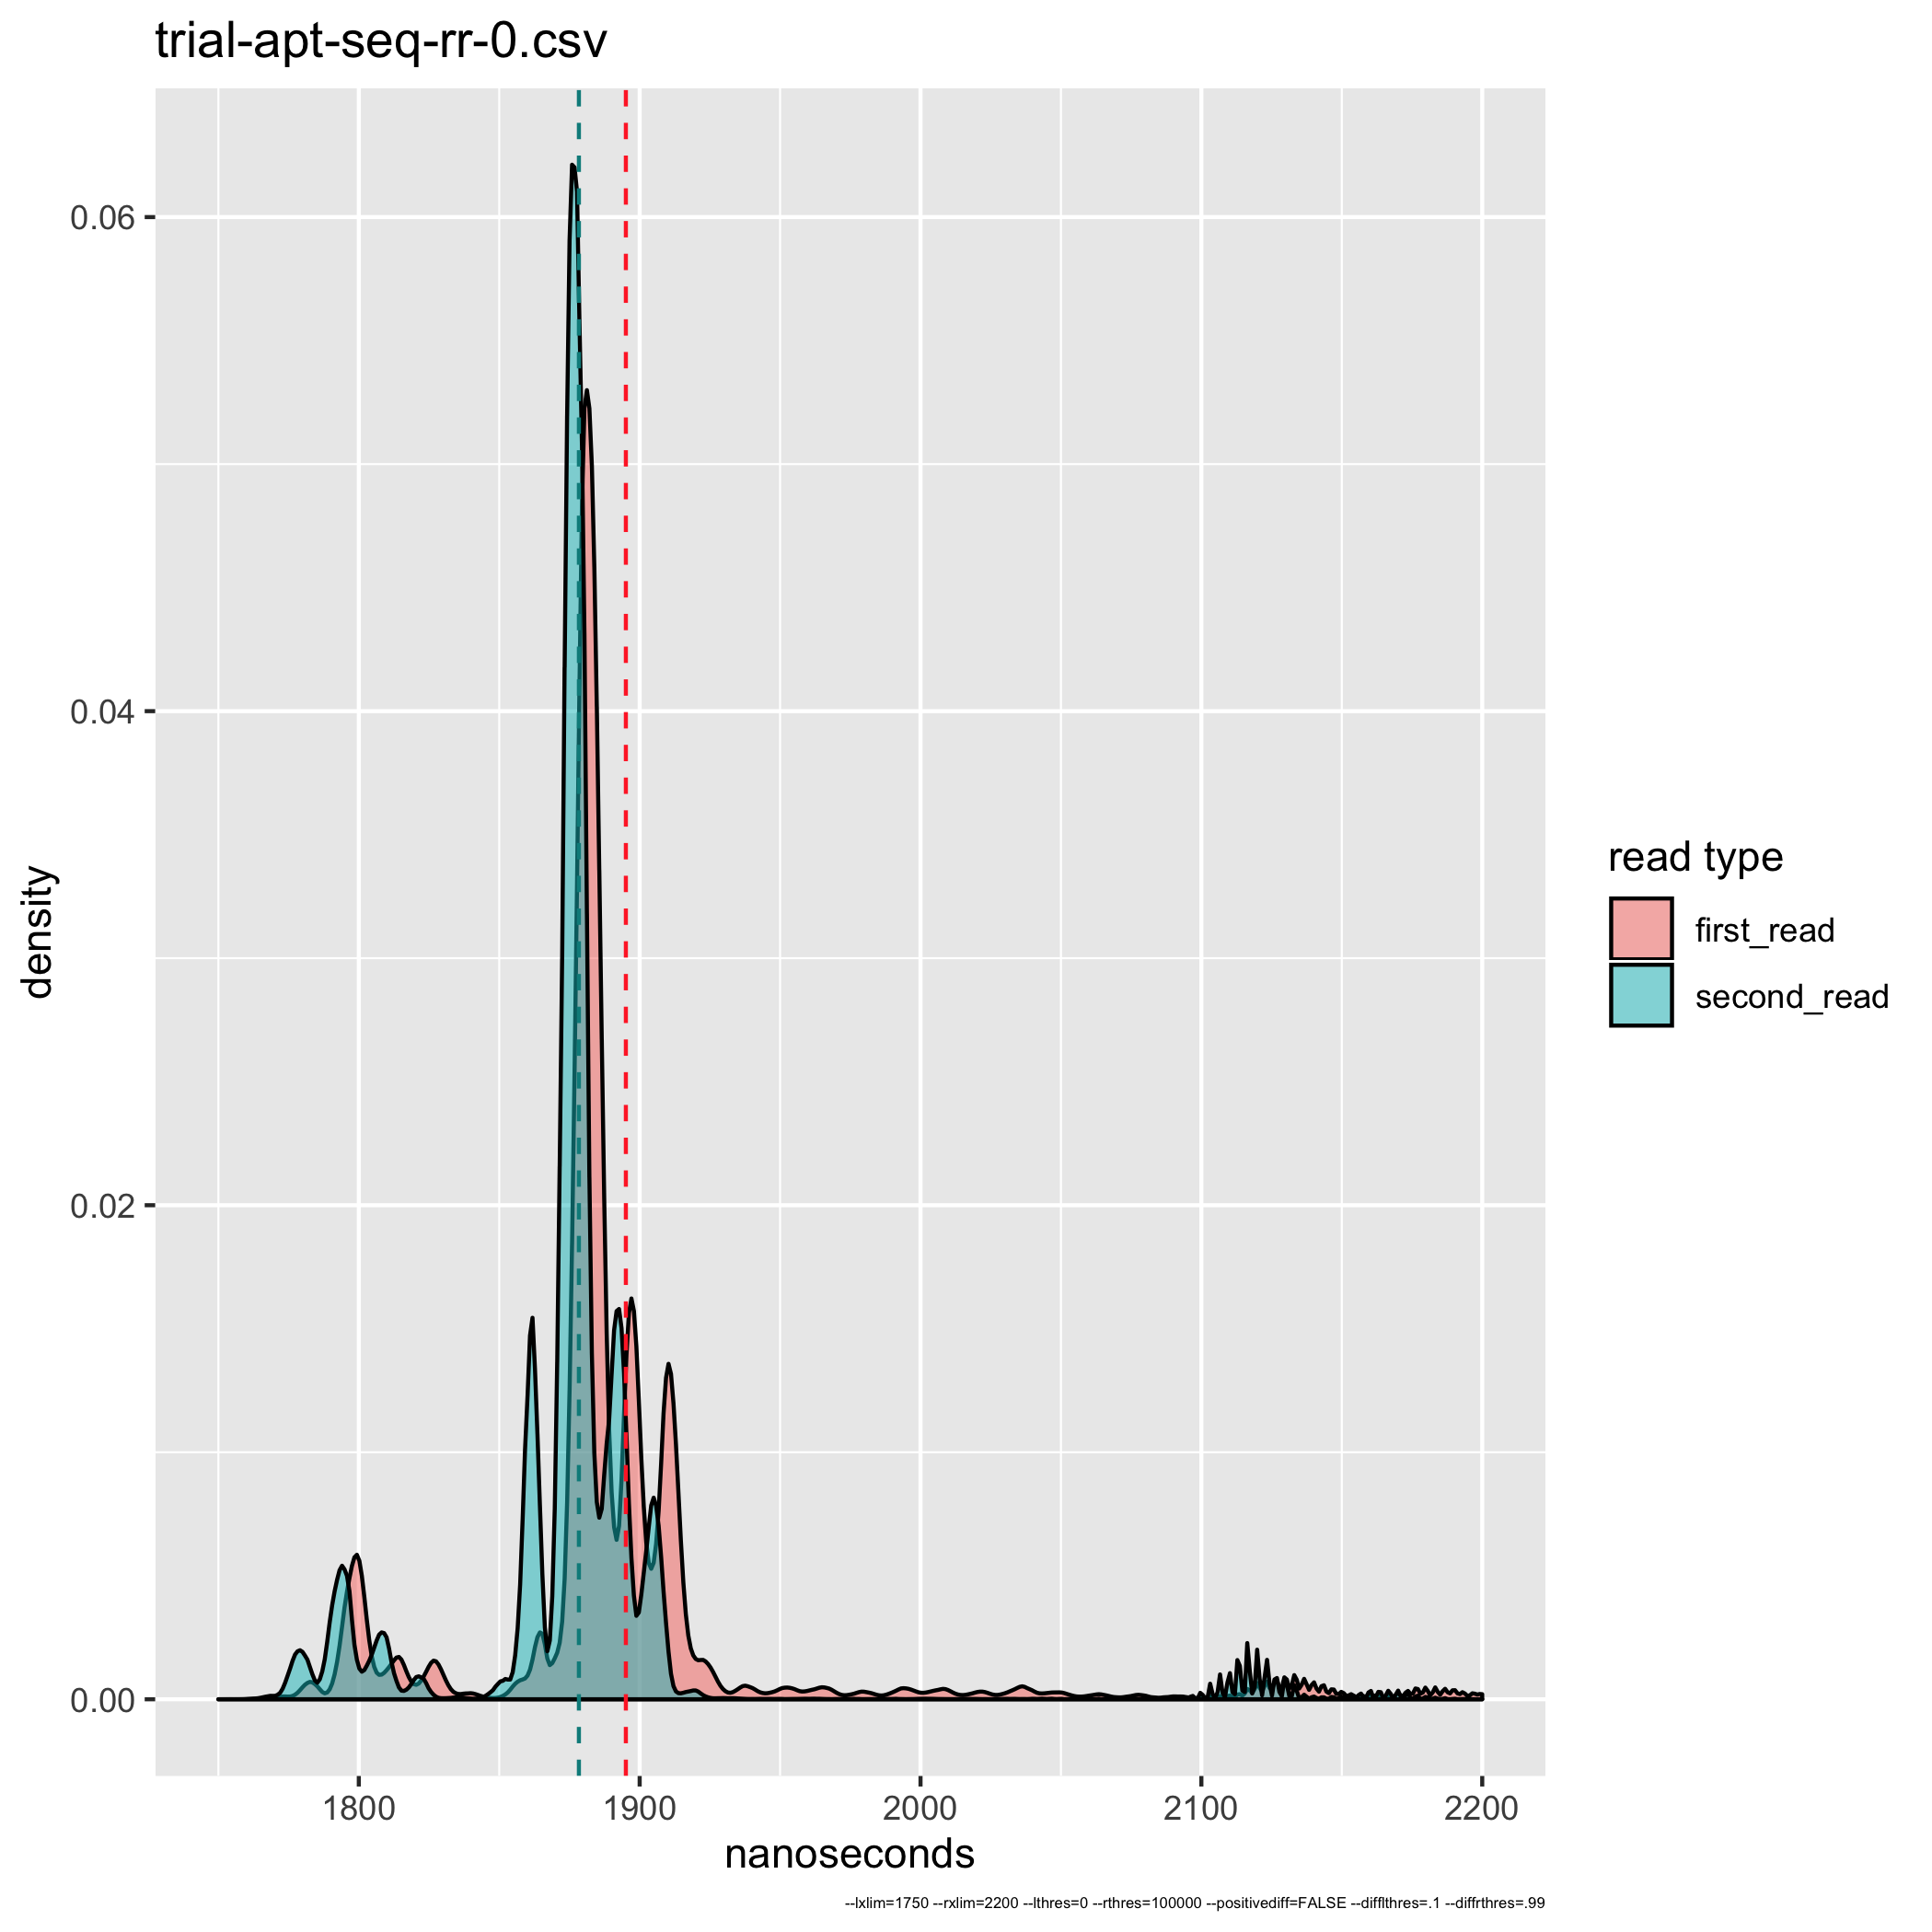
\includegraphics[width=\linewidth]{trial-apt-seq-rr-0-histogram.png}

  \end{column}
  \begin{column}{0.5\textwidth}
   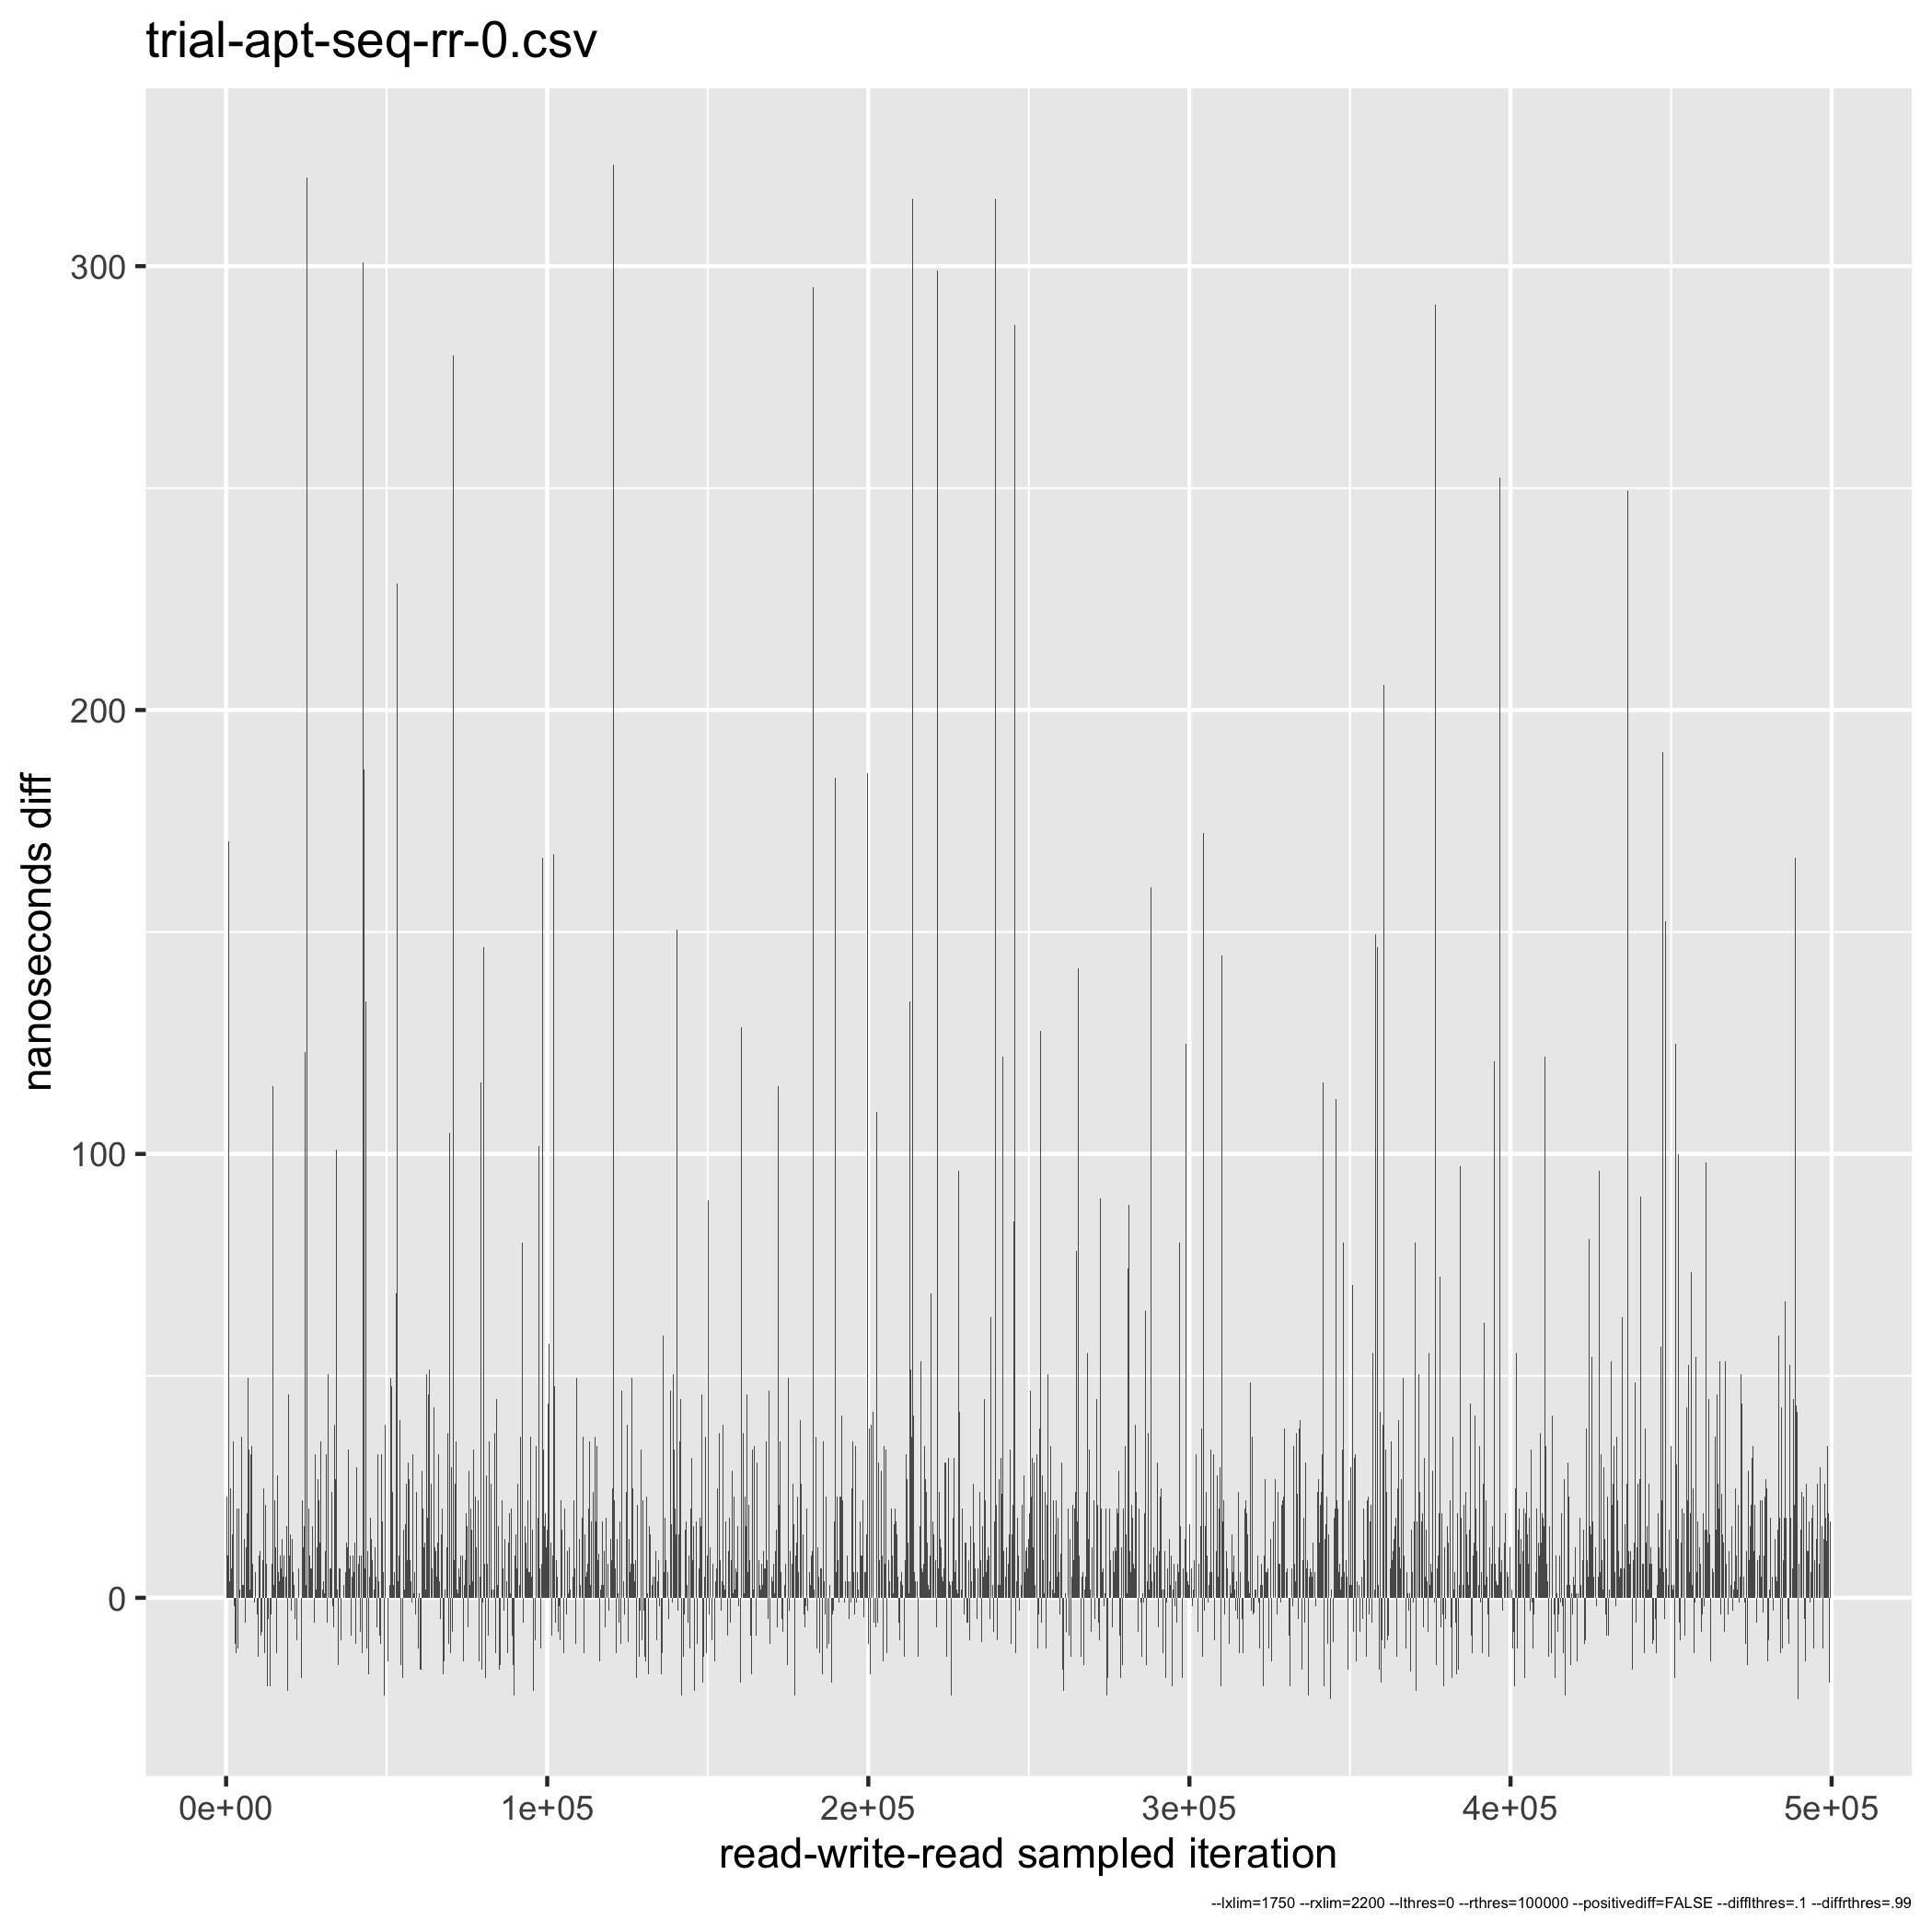
\includegraphics[width=\linewidth]{trial-apt-seq-rr-0-barchart.png}

  \end{column}

 \end{columns}

\end{frame}

\begin{frame}
 \frametitle{What Might Causes These Graphs?}
 \begin{itemize}
  \item NUMA
  \item Prefetchers
  \item CPU frequency scaling
  \item CPU power management
  \item Hyperthreading
  \item Saturated Infiniband fabrics seem to increase mean latencies and variance.
  \item Potential Infiniband pathologies?
  \item Potential DDIO pathologies (perhaps with \texttt{clflush} interactions)?
  \item RDMA-enabled nodes are likely to be network-traffic intensive (more cache evictions)
 \end{itemize}
\end{frame}

\begin{frame}
 \frametitle{Problems Moving Forward}
 \begin{itemize}
  \item The ``diff stepdown'' destroys any statistical predictions on a cache miss/miss.
  \item Noisy data is harder to predict on
  \item Many of distributions are not normal, so we cannot use common regression tools.
  \item Couldn't figure out a baseline for the ns difference between DRAM and LLC access
  \item Mapping addresses to sets was far more challenging than expected
  \item Haven't check if the compiler does anything weird
 \end{itemize}
\end{frame}


\begin{frame}
 \frametitle{Conclusion}
 \vskip0pt plus 1filll
 \begin{itemize}
  \item \textit{Probably} can predict cache misses/hits
  \item Lots of problems/pathologies you need to work through first
 \end{itemize}

 \vskip0pt plus 1filll
 \centering
 \footnotesize
 \texttt{https://github.com/emersonford/NetCAT-Replication}
 \vspace{20pt}

\end{frame}


\end{document}
